\documentclass{beamer}
\usetheme{metropolis}
\usepackage{latexsym}
\usepackage{amssymb}
\usepackage{amsbsy}
\usepackage{alltt}
\usepackage{tikz}
\usetikzlibrary{shapes}
\usepackage{stmaryrd}
\usepackage{graphicx}

\newcommand{\imp}{\Rightarrow}
\newcommand{\etal}{\textit{et. al}}
\newcommand{\adhoc}{\textit{ad hoc}}
\newcommand{\ie}{\textit{i.e.}}
\newcommand{\etc}{\textit{etc}}
\newcommand{\eg}{\textit{e.g.}}
\newcommand{\konst}[1]{\ensuremath{\mbox{\bf{#1}}}}
\newcommand{\nil}{\konst{[\,]}}
\newcommand{\cons}[2]{{#1}\boldsymbol{:}\boldsymbol{:}{#2}}
\newcommand{\hollamb}{\boldsymbol{\lambda}}
\newcommand{\itelse}[3]{\mbox{$\mbox{\tt if}\ {#1}\ \mbox{\tt then}\ {#2}\
    \mbox{\tt else}\ {#3}$}}
\newcommand{\set}[1]{\{ {#1} \}}
\newcommand{\Lang}[1]{\ensuremath{{\cal L}({#1})}}
\newcommand{\LangTheta}[1]{\ensuremath{{\mathcal L}_{\theta}({#1})}}
\newcommand{\inbox}[1] {\begin{center}
                         \framebox{\parbox{0.984\textwidth}{#1}}
                         \end{center}}
\newcommand{\den}[1]{%
  \ensuremath{%
    \left\llbracket{#1}
    \right\rrbracket}}

% for backslashes in alltt environments
\newcommand{\bs}{\texttt{\symbol{92}}}

\begin{document}

% Title page

\author{Isaac Amundson~\textsuperscript{1} \and %
Darren Cofer~\textsuperscript{1} \and %
Junaid Babar~\textsuperscript{1} \and %
Eric Mercer~\textsuperscript{2} \and %
Karl Hoech~\textsuperscript{1} \and %
David Hardin~\textsuperscript{1} \and %
%Thomas Logan~\textsuperscript{1} \and %
Johannes~{\AA}man~Pohjola~\textsuperscript{3} \and %
\underline{Konrad Slind}~\textsuperscript{1}
}

\institute{\textsuperscript{1} Collins Aerospace \and \textsuperscript{2} BYU \and \textsuperscript{3} Data61}

\date{Sept. 14, 2020}
\title{Take a SEAT: \\ Security-Enhancing Architectural Transformations}
\maketitle

\begin{frame}\frametitle{Overview}
\begin{enumerate}
\item Architectural Transformations
\item Deep Dive: Message Analysis
\item Assembling a Security Case
\end{enumerate}
\end{frame}


\section {Architectural Transformations}

\begin{frame}\frametitle{System Architecture}
\begin{itemize}

\item System architecture models provide a high-level setting in which
  the \emph{whole picture} of a system can be surveyed

\item A place where existing implementations, new design features, high-level
  requirements, implementations, and verifications can be combined.

\item In the DARPA \textbf{CASE} project we are developing the idea of
  \emph{Security-Enhancing} transformations on such architectural
  descriptions.

\item The goal is to develop architectural models for existing
  (legacy) systems, and then improve system security by applying architectural
  transformations

\end{itemize}

\end{frame}

\begin{frame}\frametitle{Architecture Transformations}

We have been developing a collection of
\emph{architecture-to-architecture} maps that can be applied to
provably \emph{increase} the security of a system.

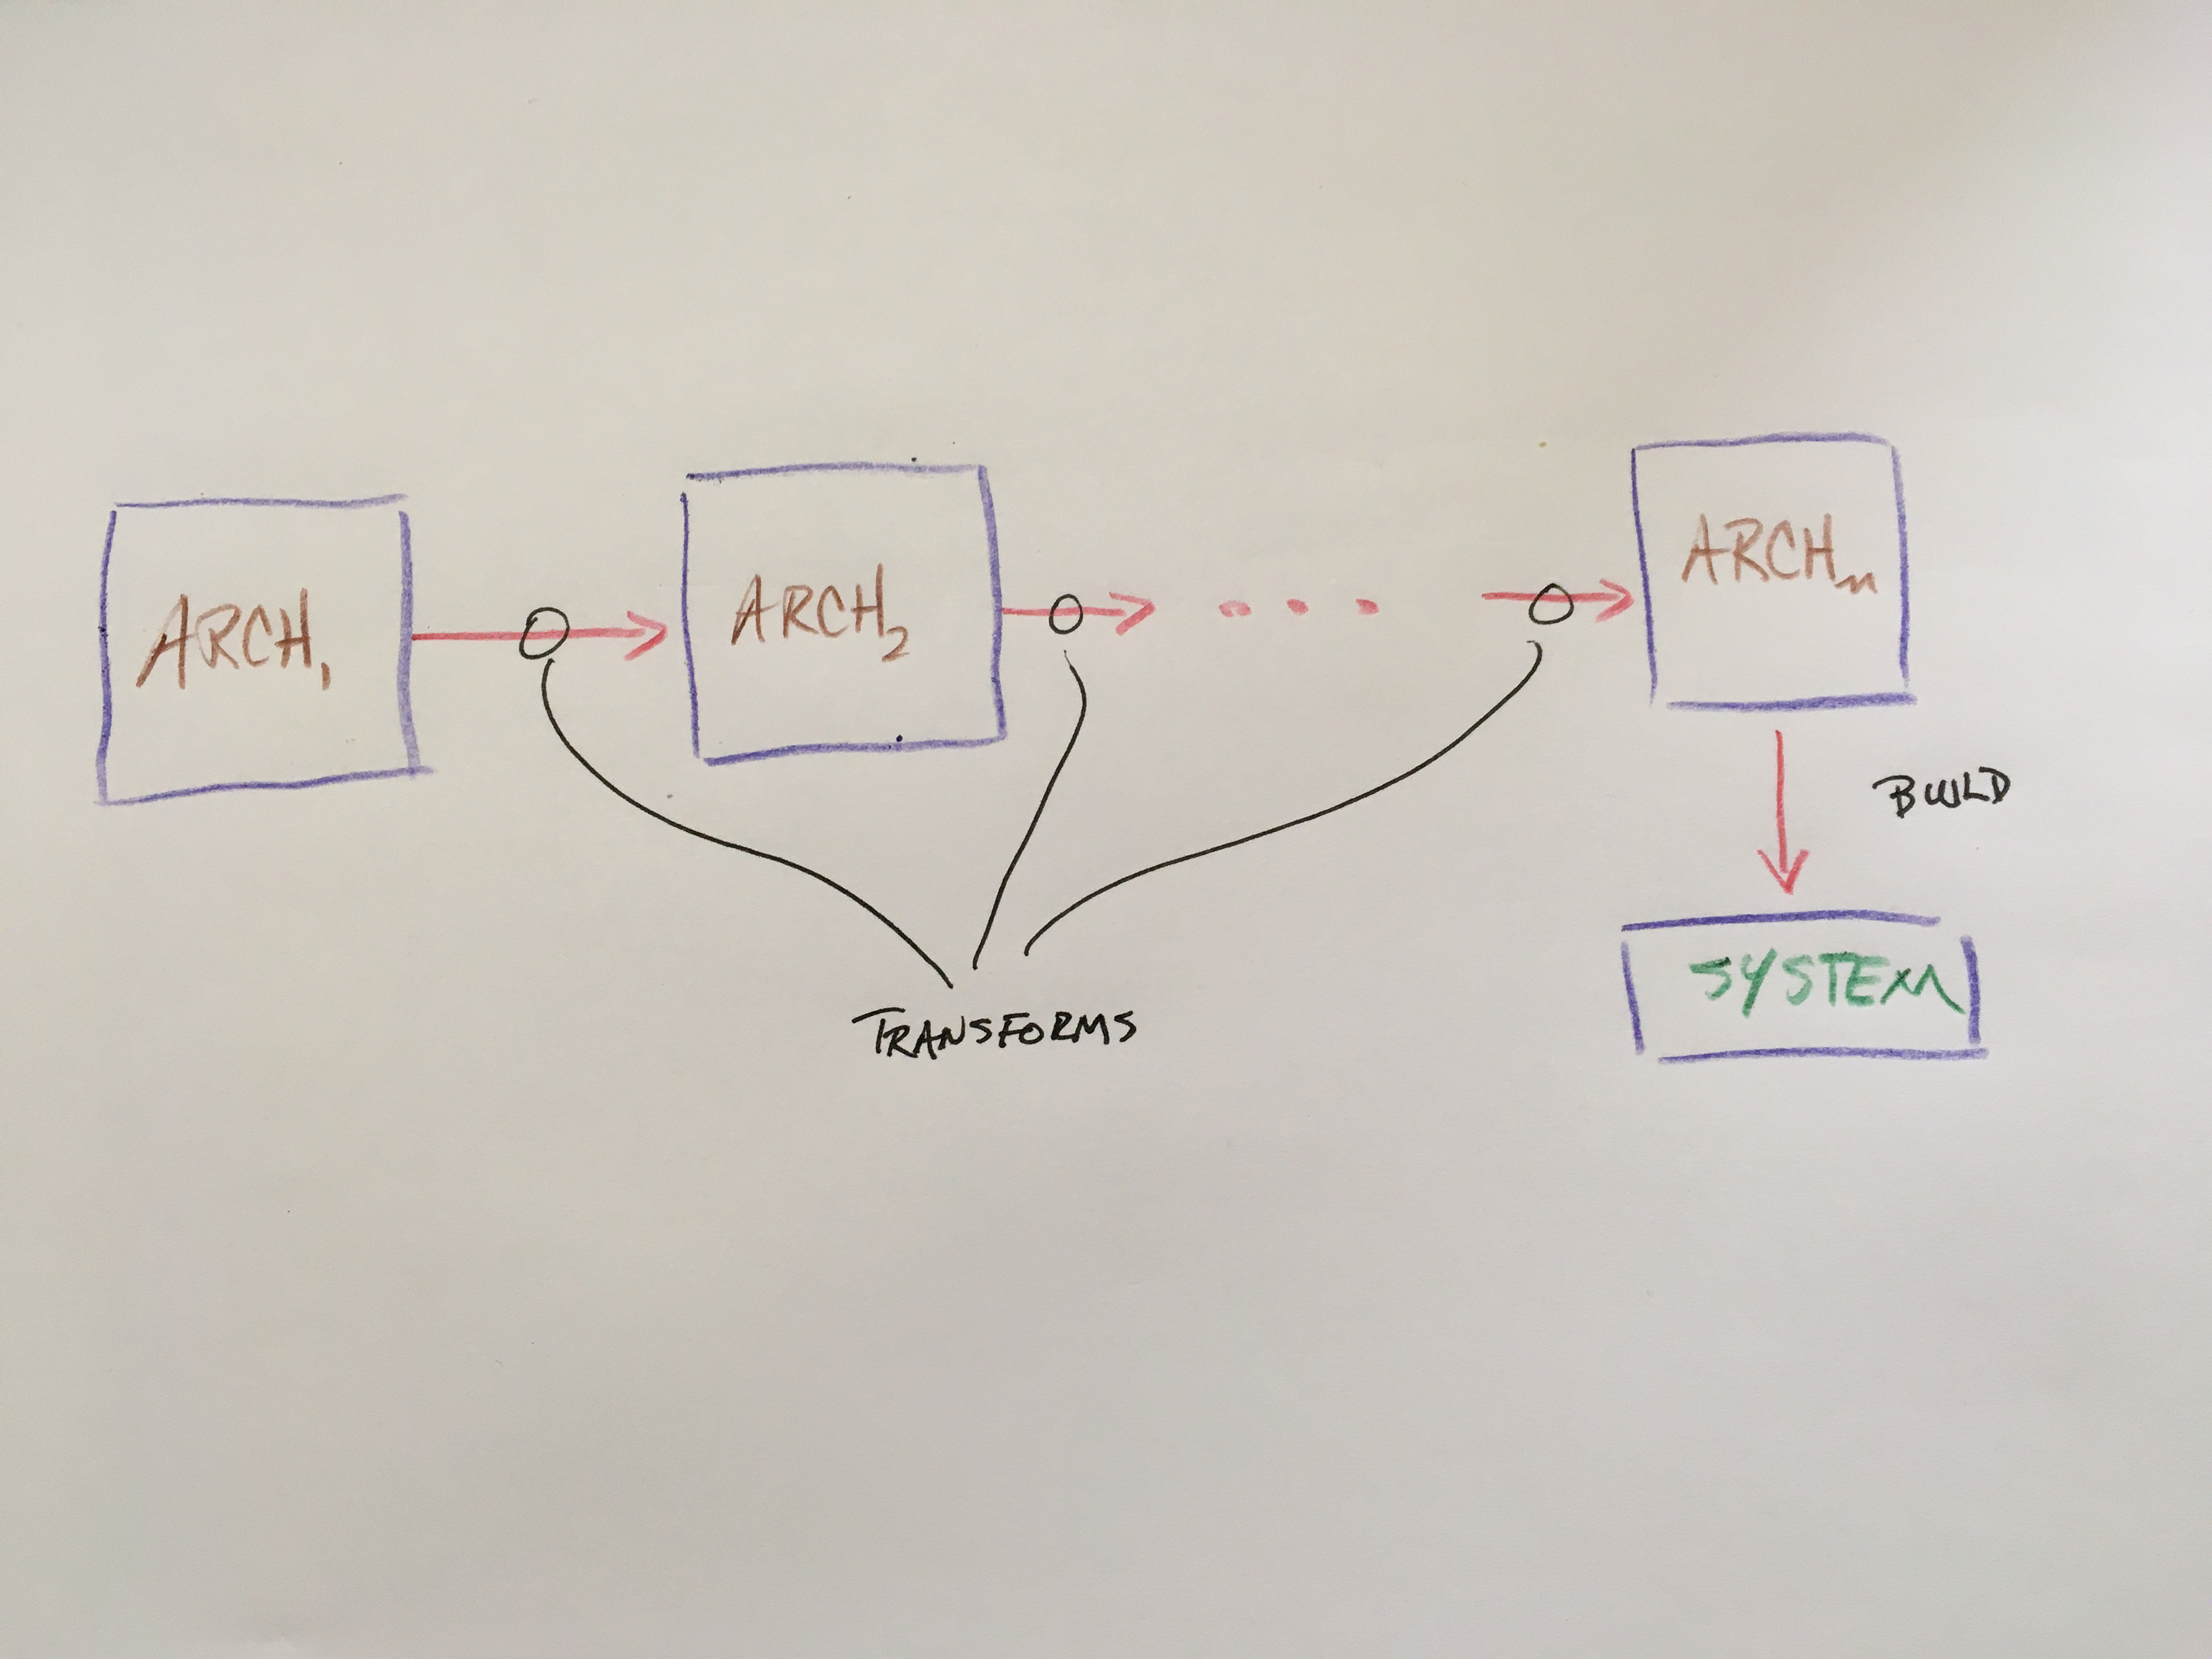
\includegraphics[width=90mm,height=50mm]{arch-trans.jpg}

\end{frame}

\begin{frame}\frametitle{AADL}

\begin {itemize}
\item Expressive: allows specification of
\begin{itemize}
     \item memory and buses
     \item software (types + behavior)
     \item communication
     \item scheduling
     \item  hierarchical organization of components
\end{itemize}
\item Tool support in Eclipse (via OSATE)
\item Extensible via \emph{annexes}
\item At Collins we have developed two annexes being used on CASE
\begin{itemize}
\item AGREE  (Assume-Guarantee contracts on components)
\item Resolute (Assurance cases)
\end{itemize}
\end{itemize}
\end{frame}


\begin{frame}\frametitle{Transformation: Message Filtering}

A \emph{filter} is conceptually very simple: it checks validity of its input data.
If the data is valid, then it is passed on. Otherwise it is dropped.

\hspace*{10mm}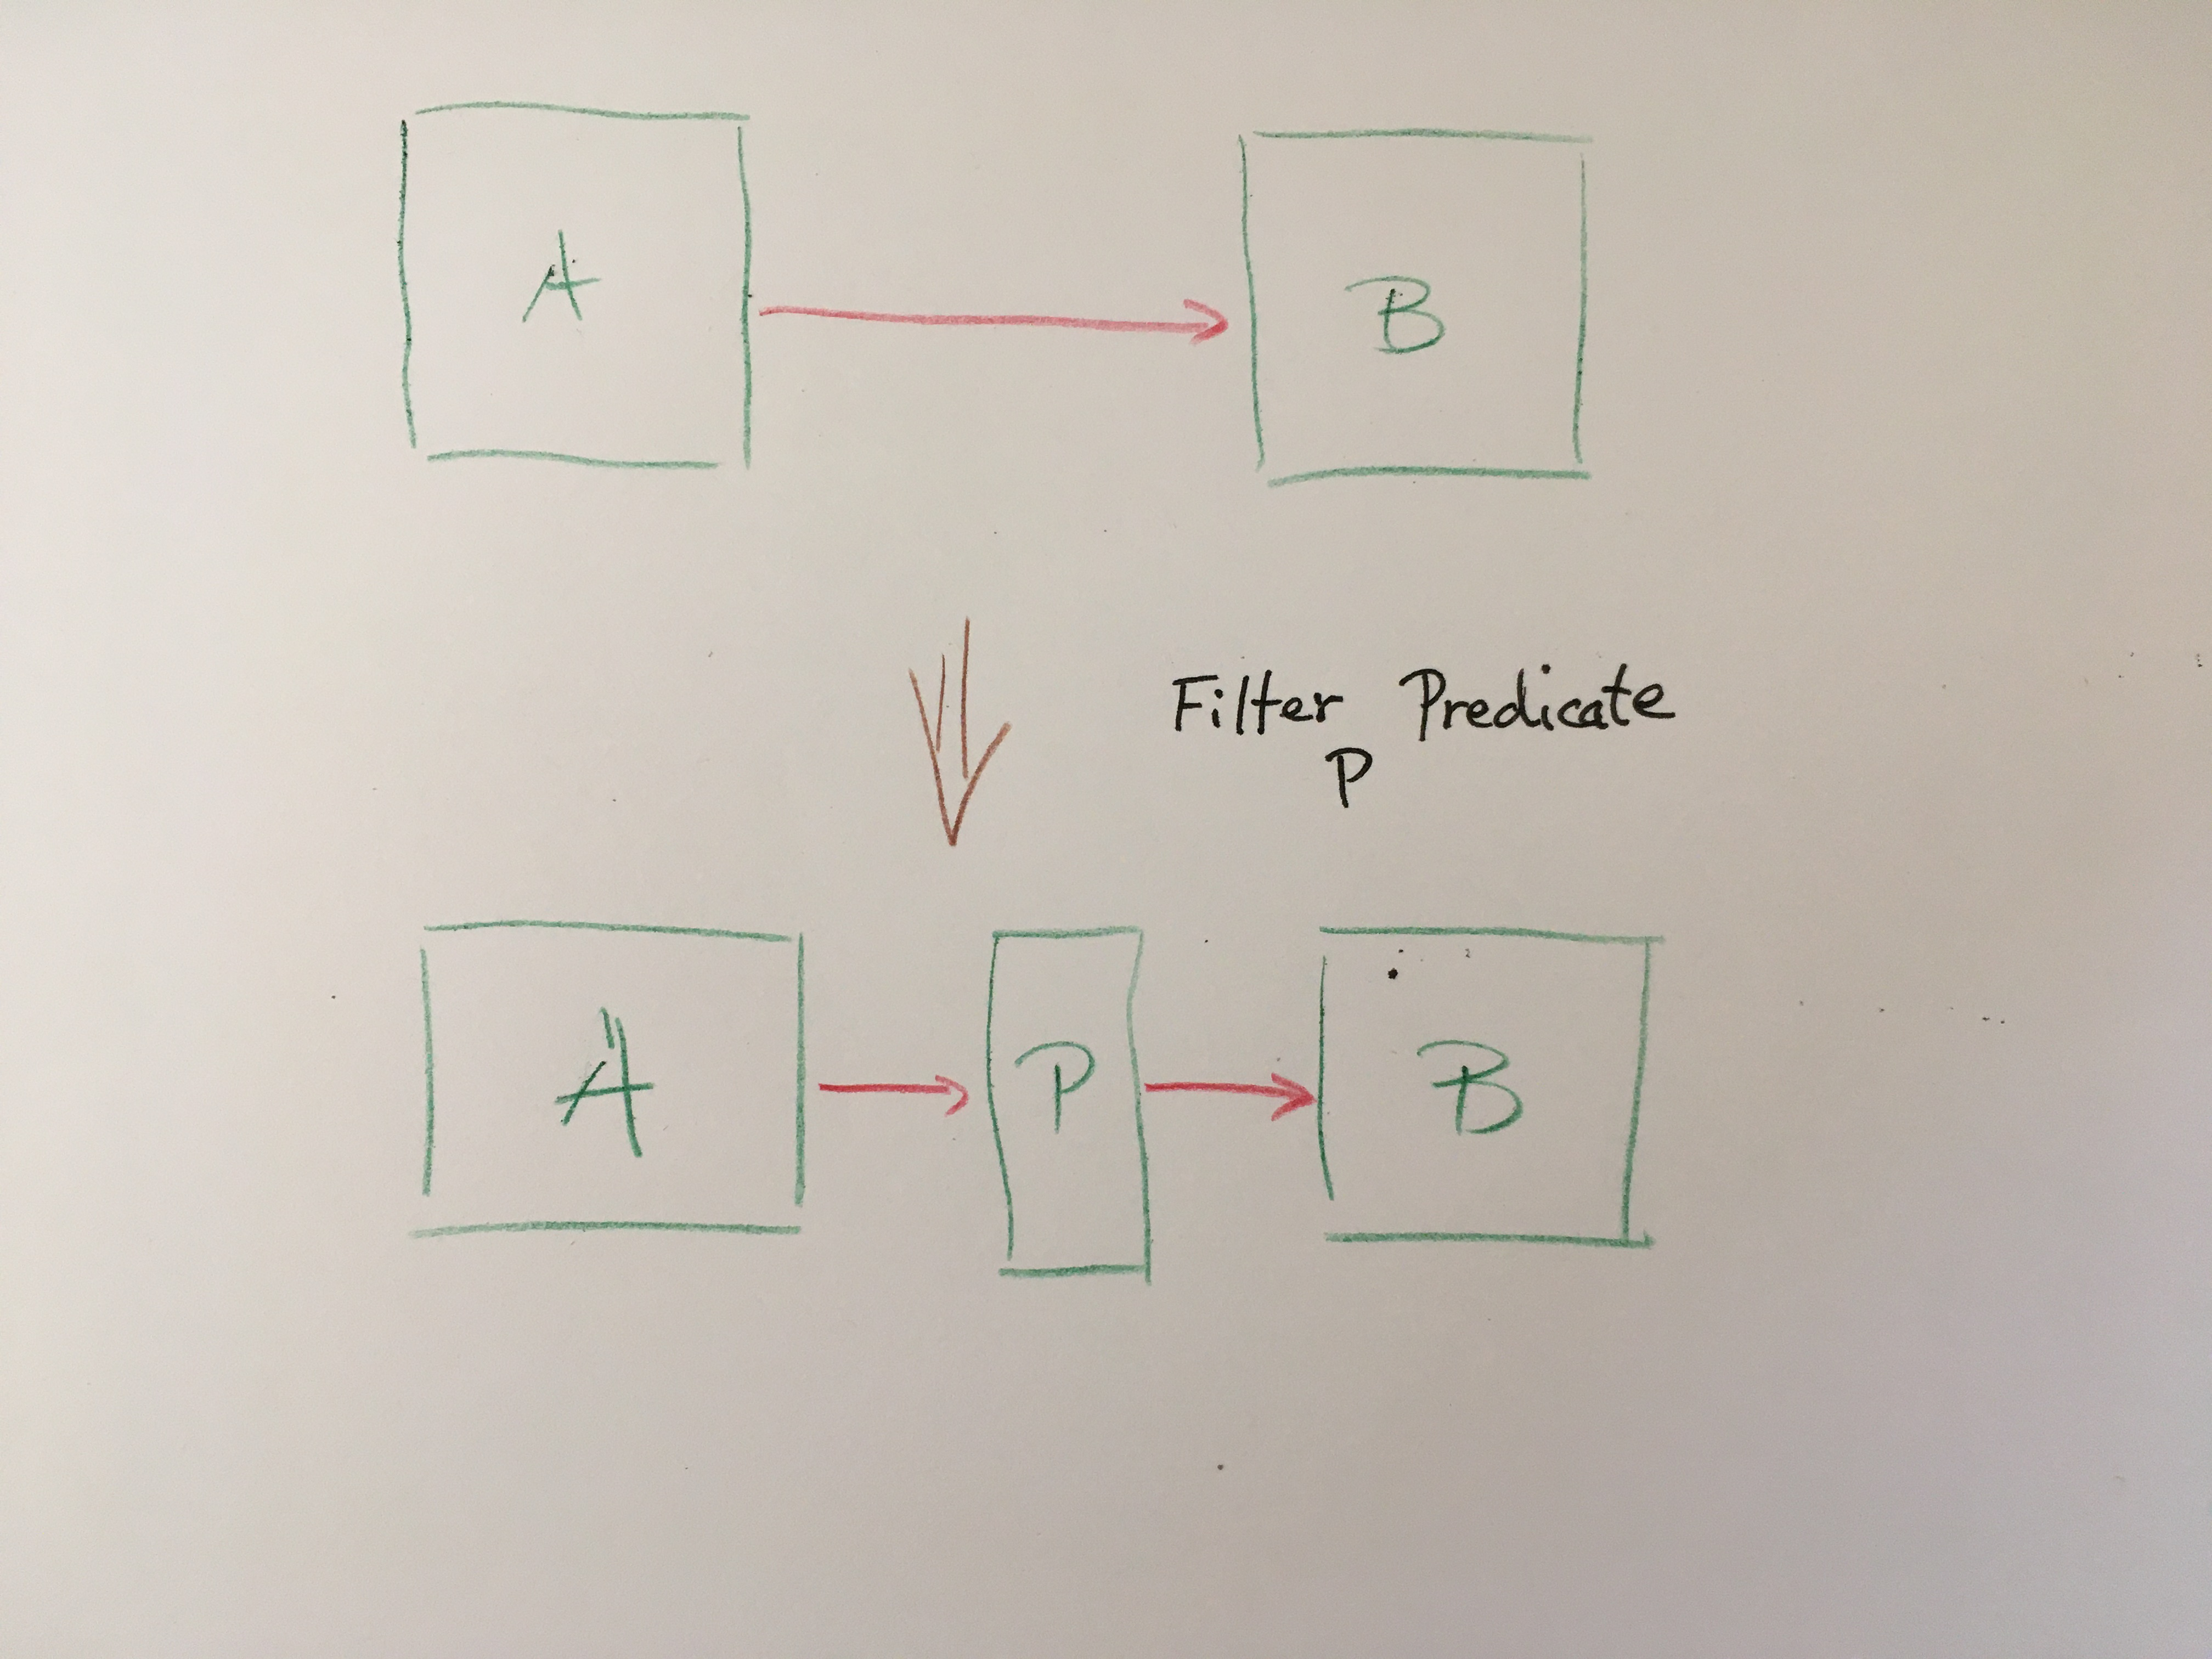
\includegraphics[width=90mm,height=50mm]{filter.jpg}

\end{frame}


\begin{frame}\frametitle{Transformation: Message Monitoring}

A \emph{monitor} checks to see that a relationship $\mathcal{R}$ holds
over a collection of message streams through time. If the
specification is violated, an \emph{alert} is sent out.

\begin{itemize}
  \item We currently use past-time temporal logic to specify monitors
\end{itemize}

\hspace*{10mm}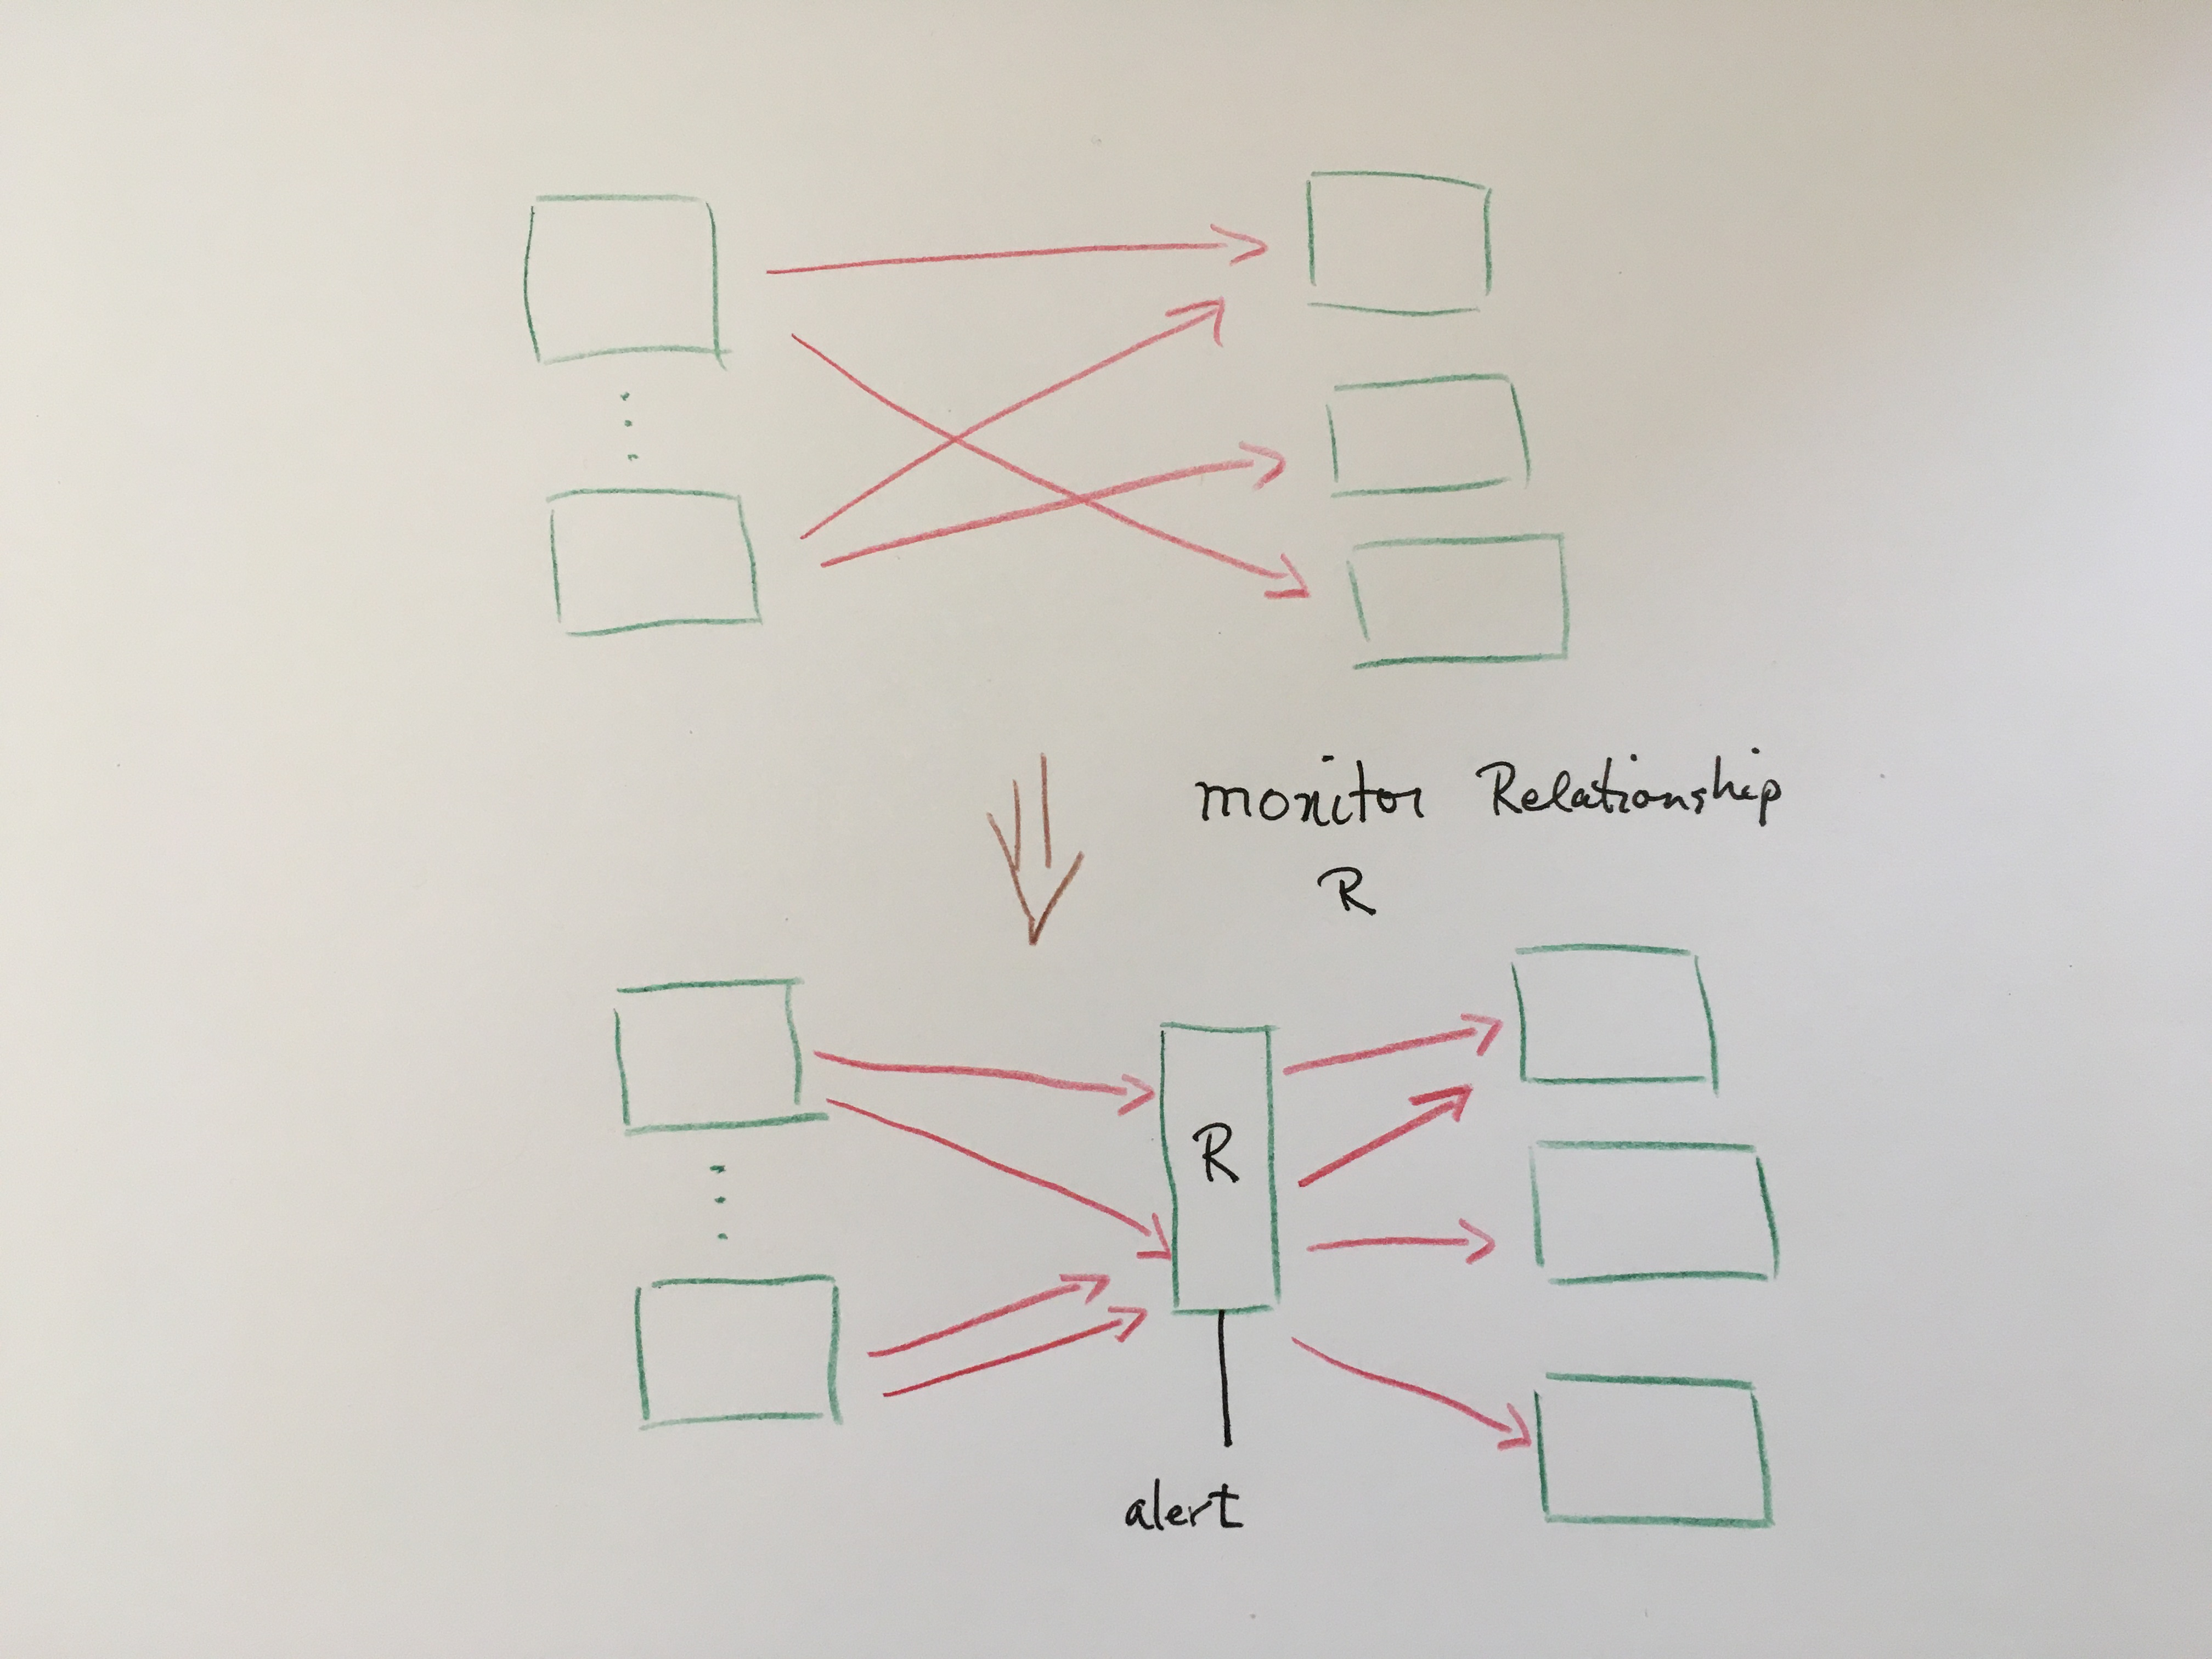
\includegraphics[width=90mm,height=40mm]{monitor.jpg}

\end{frame}


\begin{frame}\frametitle{Transformation: Isolation of `at risk' components}

An unprotected computational element can be \emph{memory protected} by
transparently lifting it out of its context and mediating access via seL4.

\hspace*{10mm}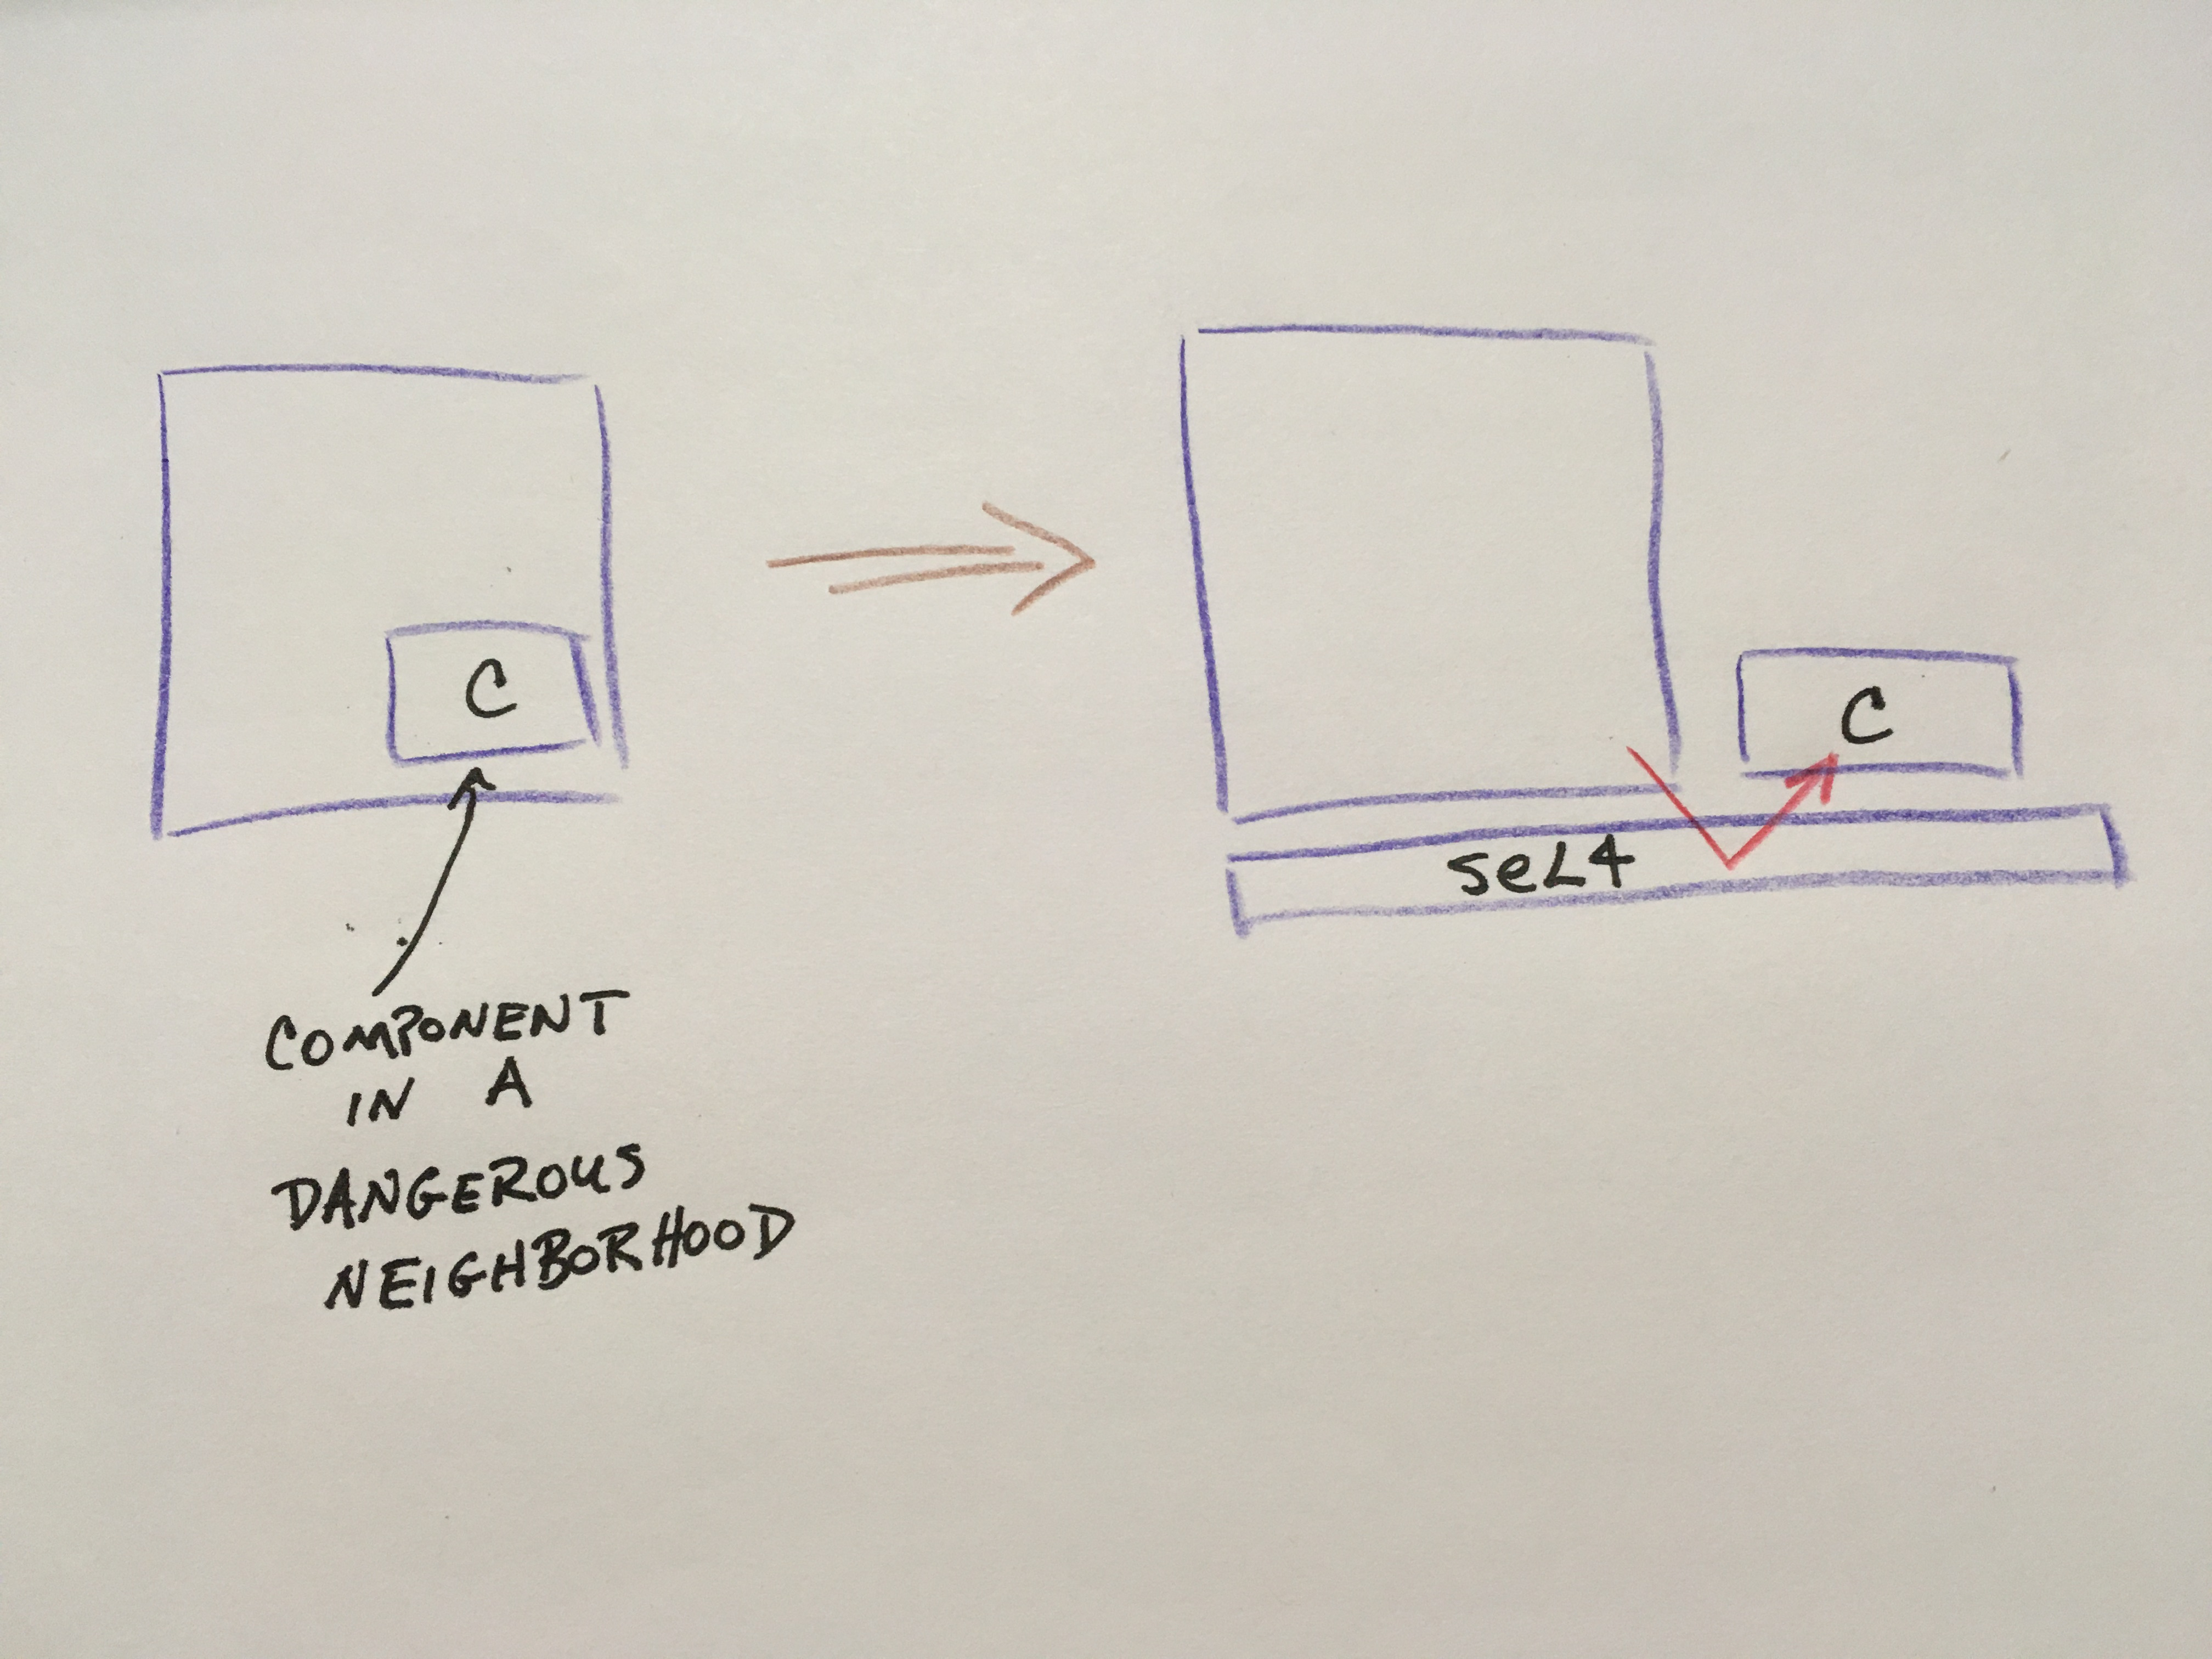
\includegraphics[width=90mm,height=40mm]{vm.jpg}

\end{frame}

\begin{frame}\frametitle{Transformation: Attestation}

Attestation inserts measurement mechanisms into a system. These
examine various aspects of system behavior, and send summaries back to
an observer system.

\hspace*{10mm}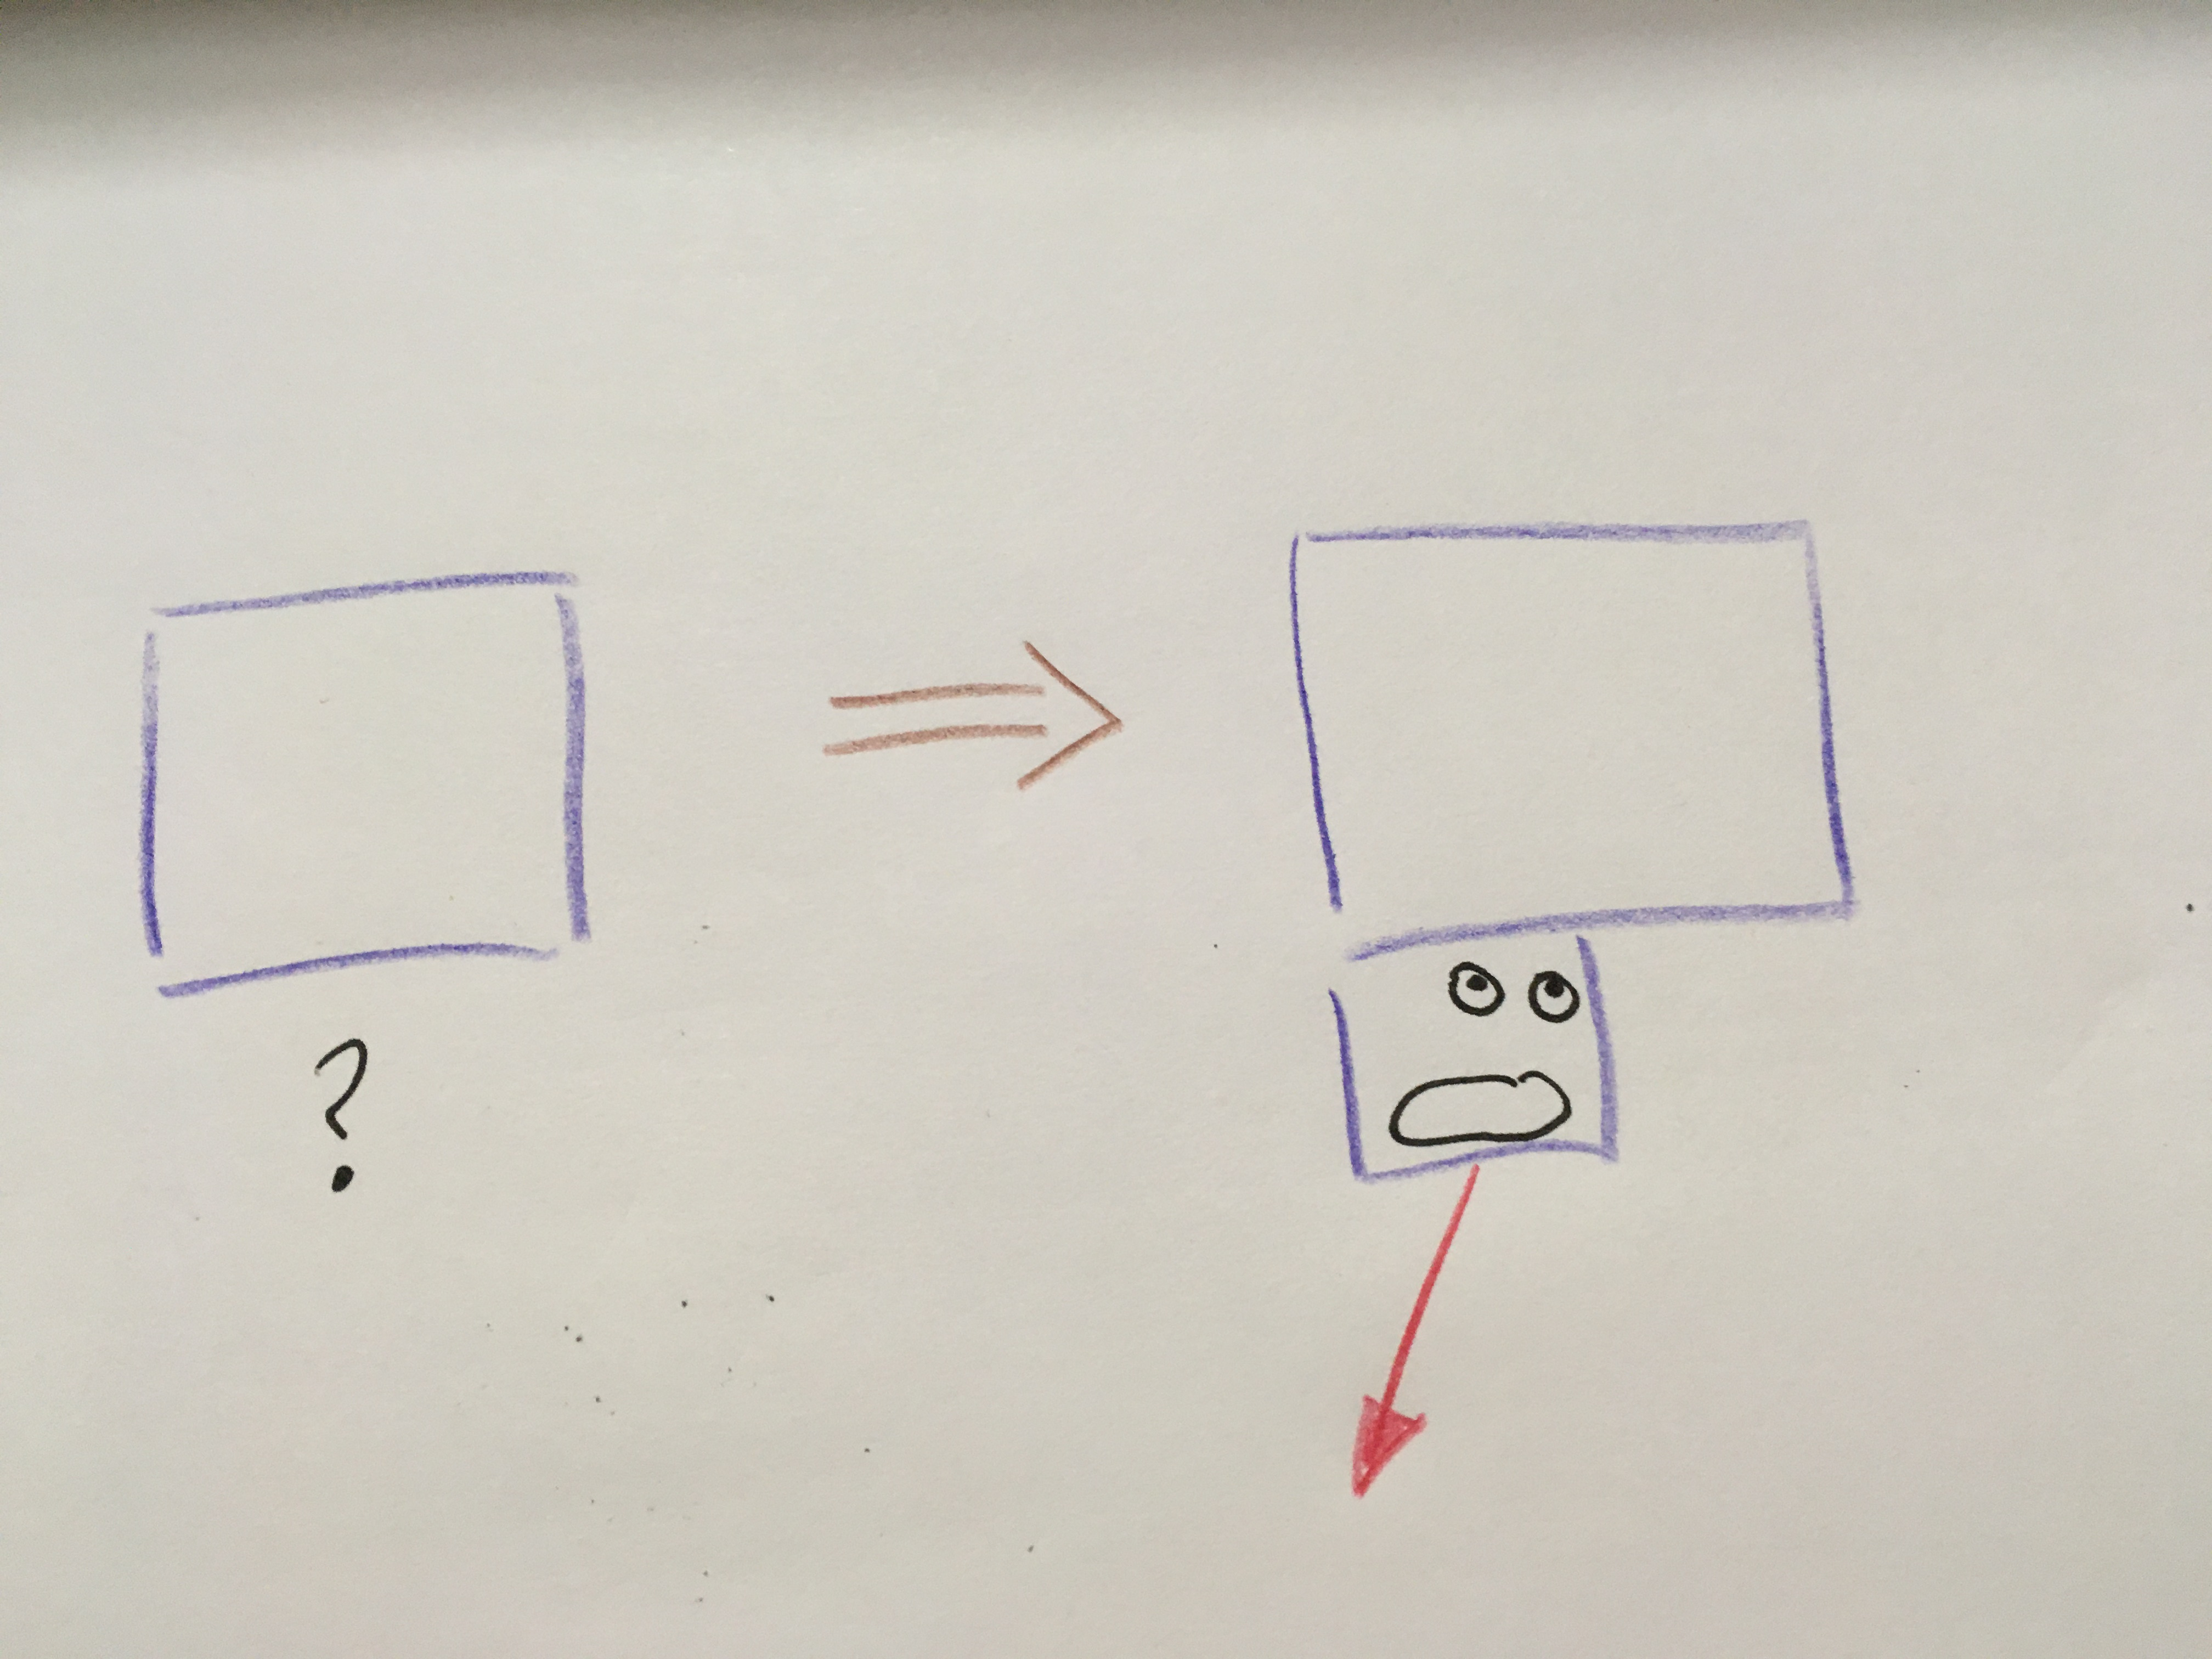
\includegraphics[width=90mm,height=40mm]{att.jpg}

\end{frame}

\begin{frame}[fragile]\frametitle{Example: uxAS}

 Current example we have been using is \textbf{uxAS}, a framework for
creating autonomous aerial systems from AFRL.

\begin{verbatim}
  https://github.com/afrl-rq/OpenUxAS
\end{verbatim}

\begin{itemize}
\item Open Source
\item Previous experience during the AFRL Summer of Innovation
\item Good setting in which to exercise our ideas
\end{itemize}

\end{frame}

\begin{frame}\frametitle{uxAS system architecture}

The initial system model we start from :

  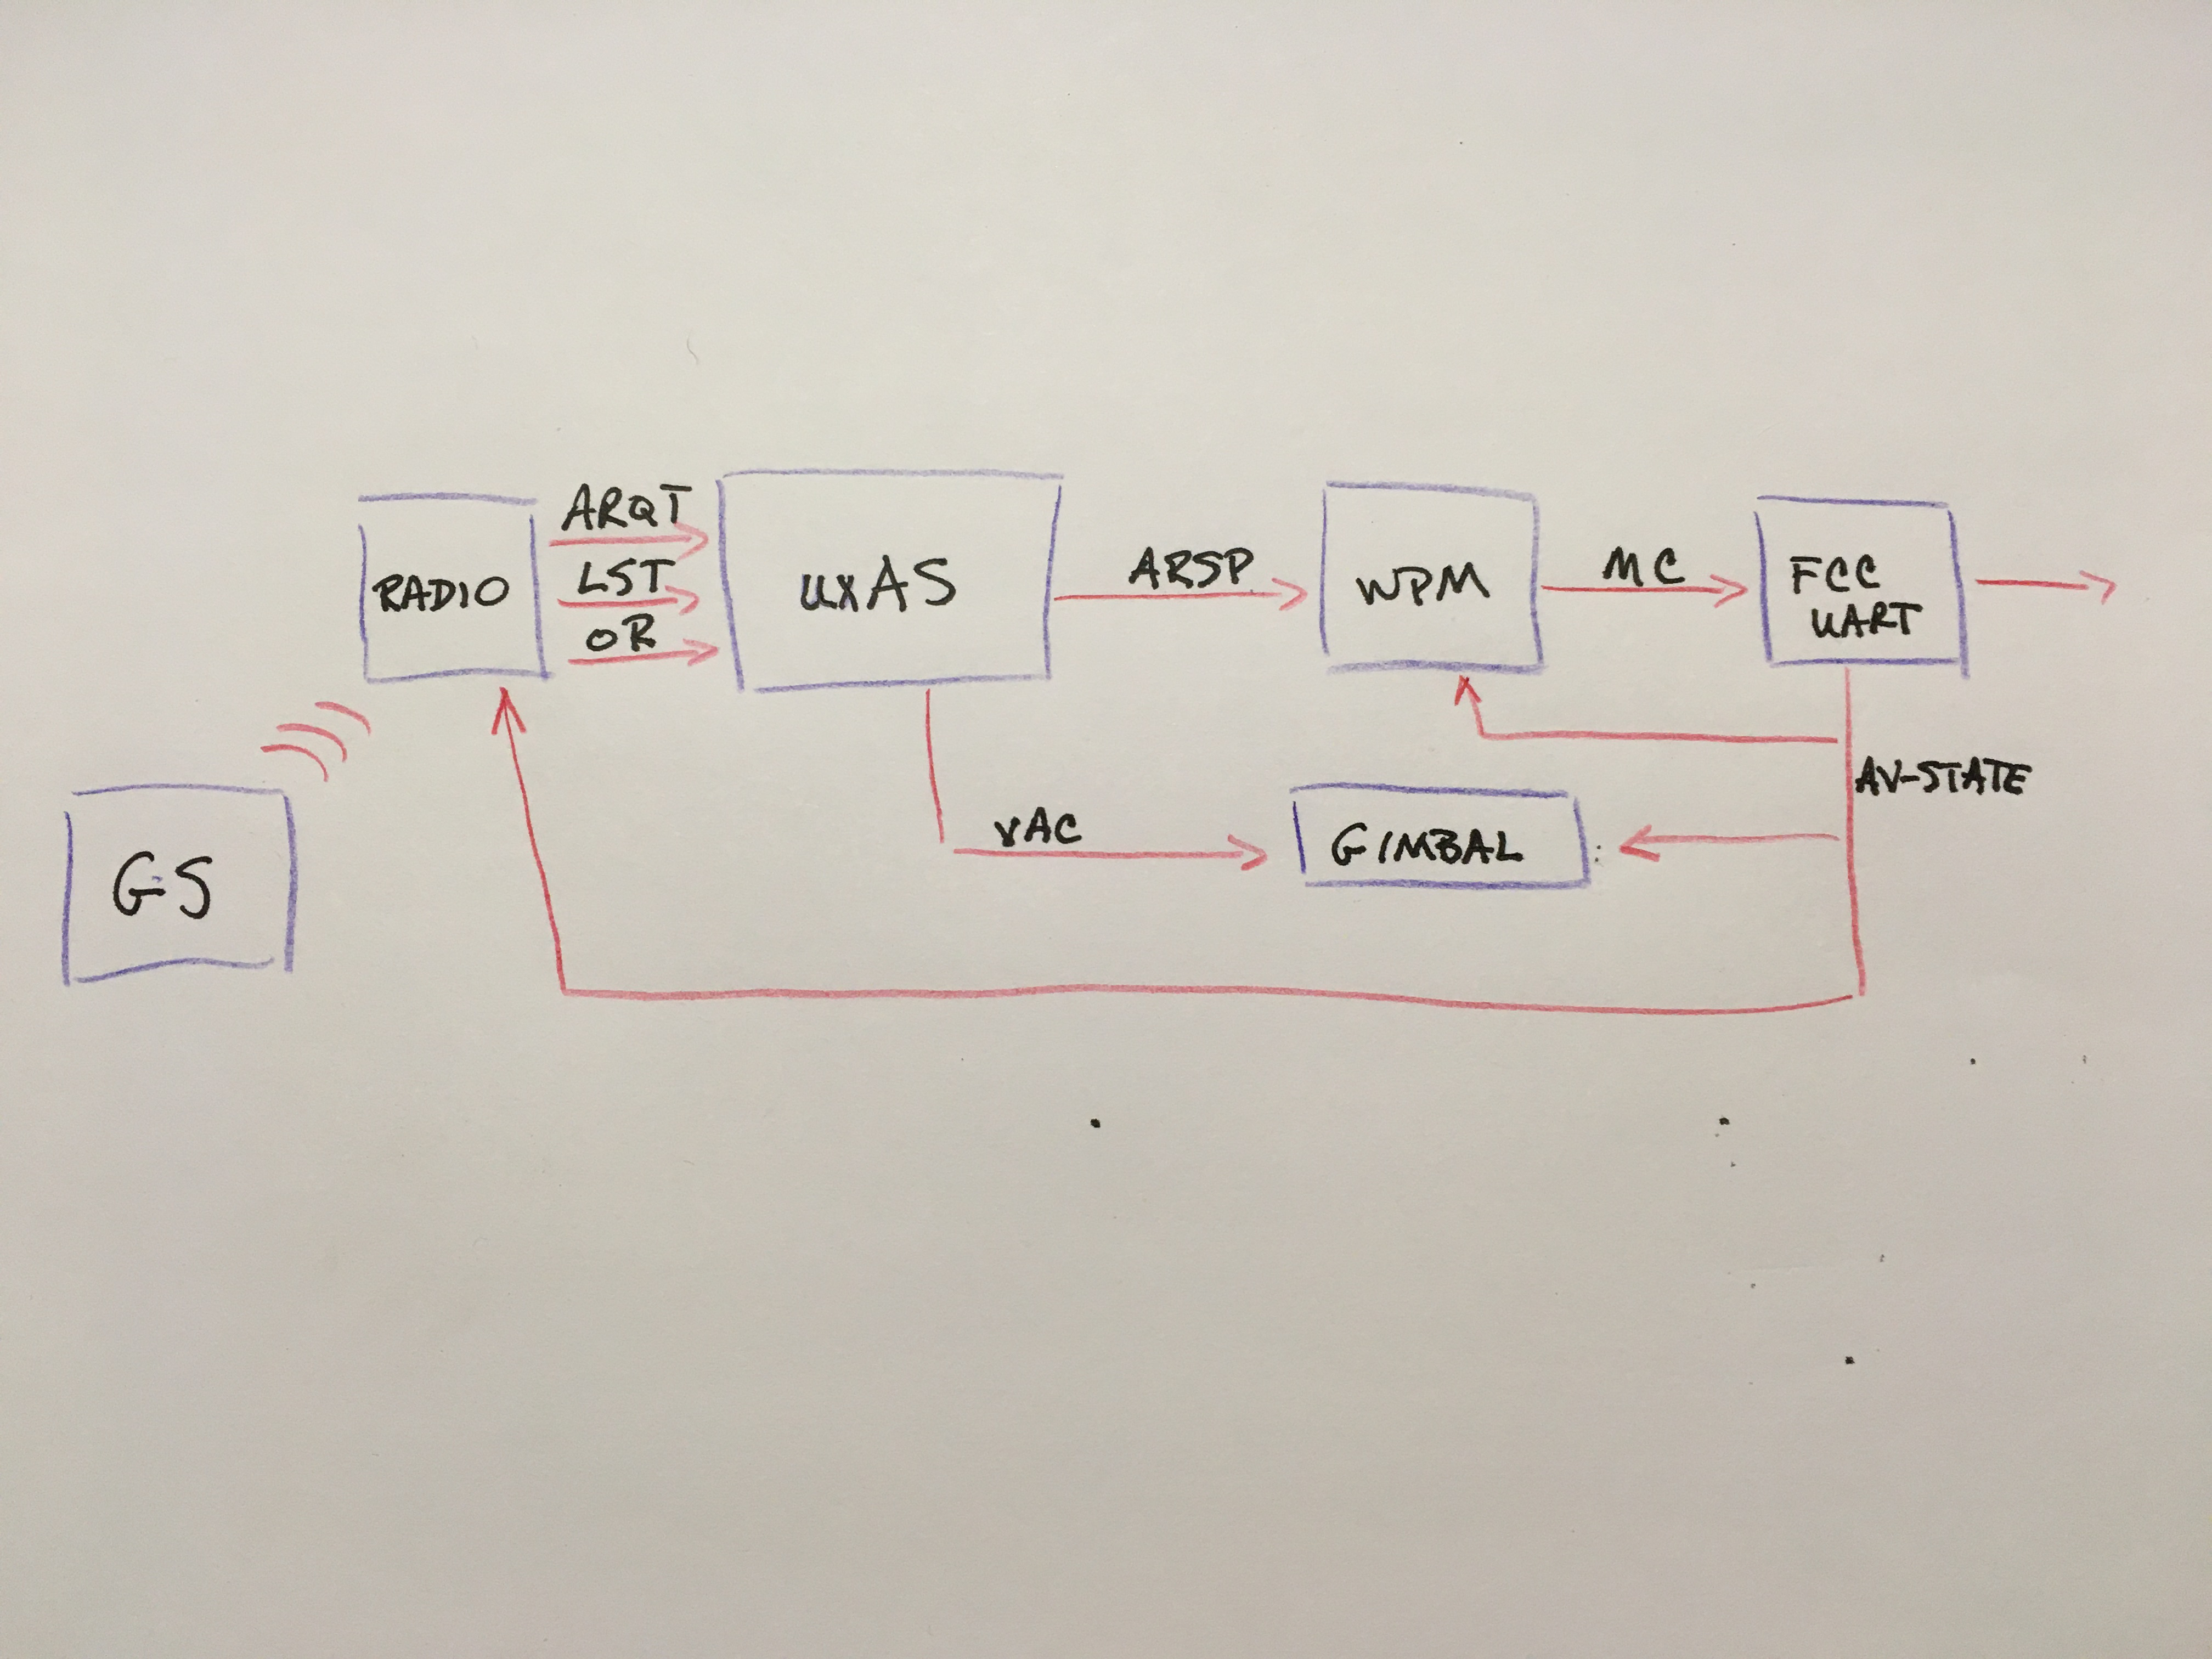
\includegraphics[width=90mm,height=50mm]{uxas-orig.jpg}


\end{frame}

\begin{frame}\frametitle{Notes on the model}

\begin{itemize}
\item UAV is preloaded with a collection of Operating Regions (Keep-in and Keep-out zones)
\item Commands from GS:
\begin{itemize}
  \item OR : set focus of operations to be the area denoted by the OR identifier
  \item LST : LineSearchTask: \emph{Follow the given sequence of points}
  \item ARQT : AutomationRequest: \emph{Create a flight plan to
    achieve a high-level description, e.g., ``surveil the given OR in
    a grid pattern''}
  \item ARSP : Response to an ARQT
  \item VAC : VehicleActionCommand
  \item MC : MissionCommand
  \item AV-State: AirVehicleState
\end{itemize}
\end{itemize}

\end{frame}

\begin{frame}\frametitle{Security Considerations}

\begin{enumerate}
\item An OR message should designate a known region
\item Each point in a LST should be a valid GPS coordinate
\item Each point in an ARSP should be in a keep-in zone and not in a keep-out zone
\item Every point in an ARSP should be a valid GPS coord
\item Every ARQT should have a corresponding ARSP
\item uxAS software is open source and could be compromised
\item Ground station could be compromised; UAV needs to defend against that
\end{enumerate}

\end{frame}

\begin{frame}\frametitle{Transformations}

\begin{enumerate}
\item (Filter) An OR message should designate a known region
\item (Filter) Each point in a LST should be a valid GPS coordinate
\item (Filter) Each point in an ARSP should be in a keep-in zone and not in a keep-out zone
\item (Filter) Every point in an Automation Response should be a valid GPS coord
\item (Monitor) Every Automation Request message should have a corresponding Automation Response
            message
\item (VM) uxAS software is open source and could be compromised,
      therefore compromising the Waypoint Manager
\item (Attestation) Ground station could be compromised
\end{enumerate}

\end{frame}

\begin{frame}\frametitle{Transformed uxAS}

The transformed model :

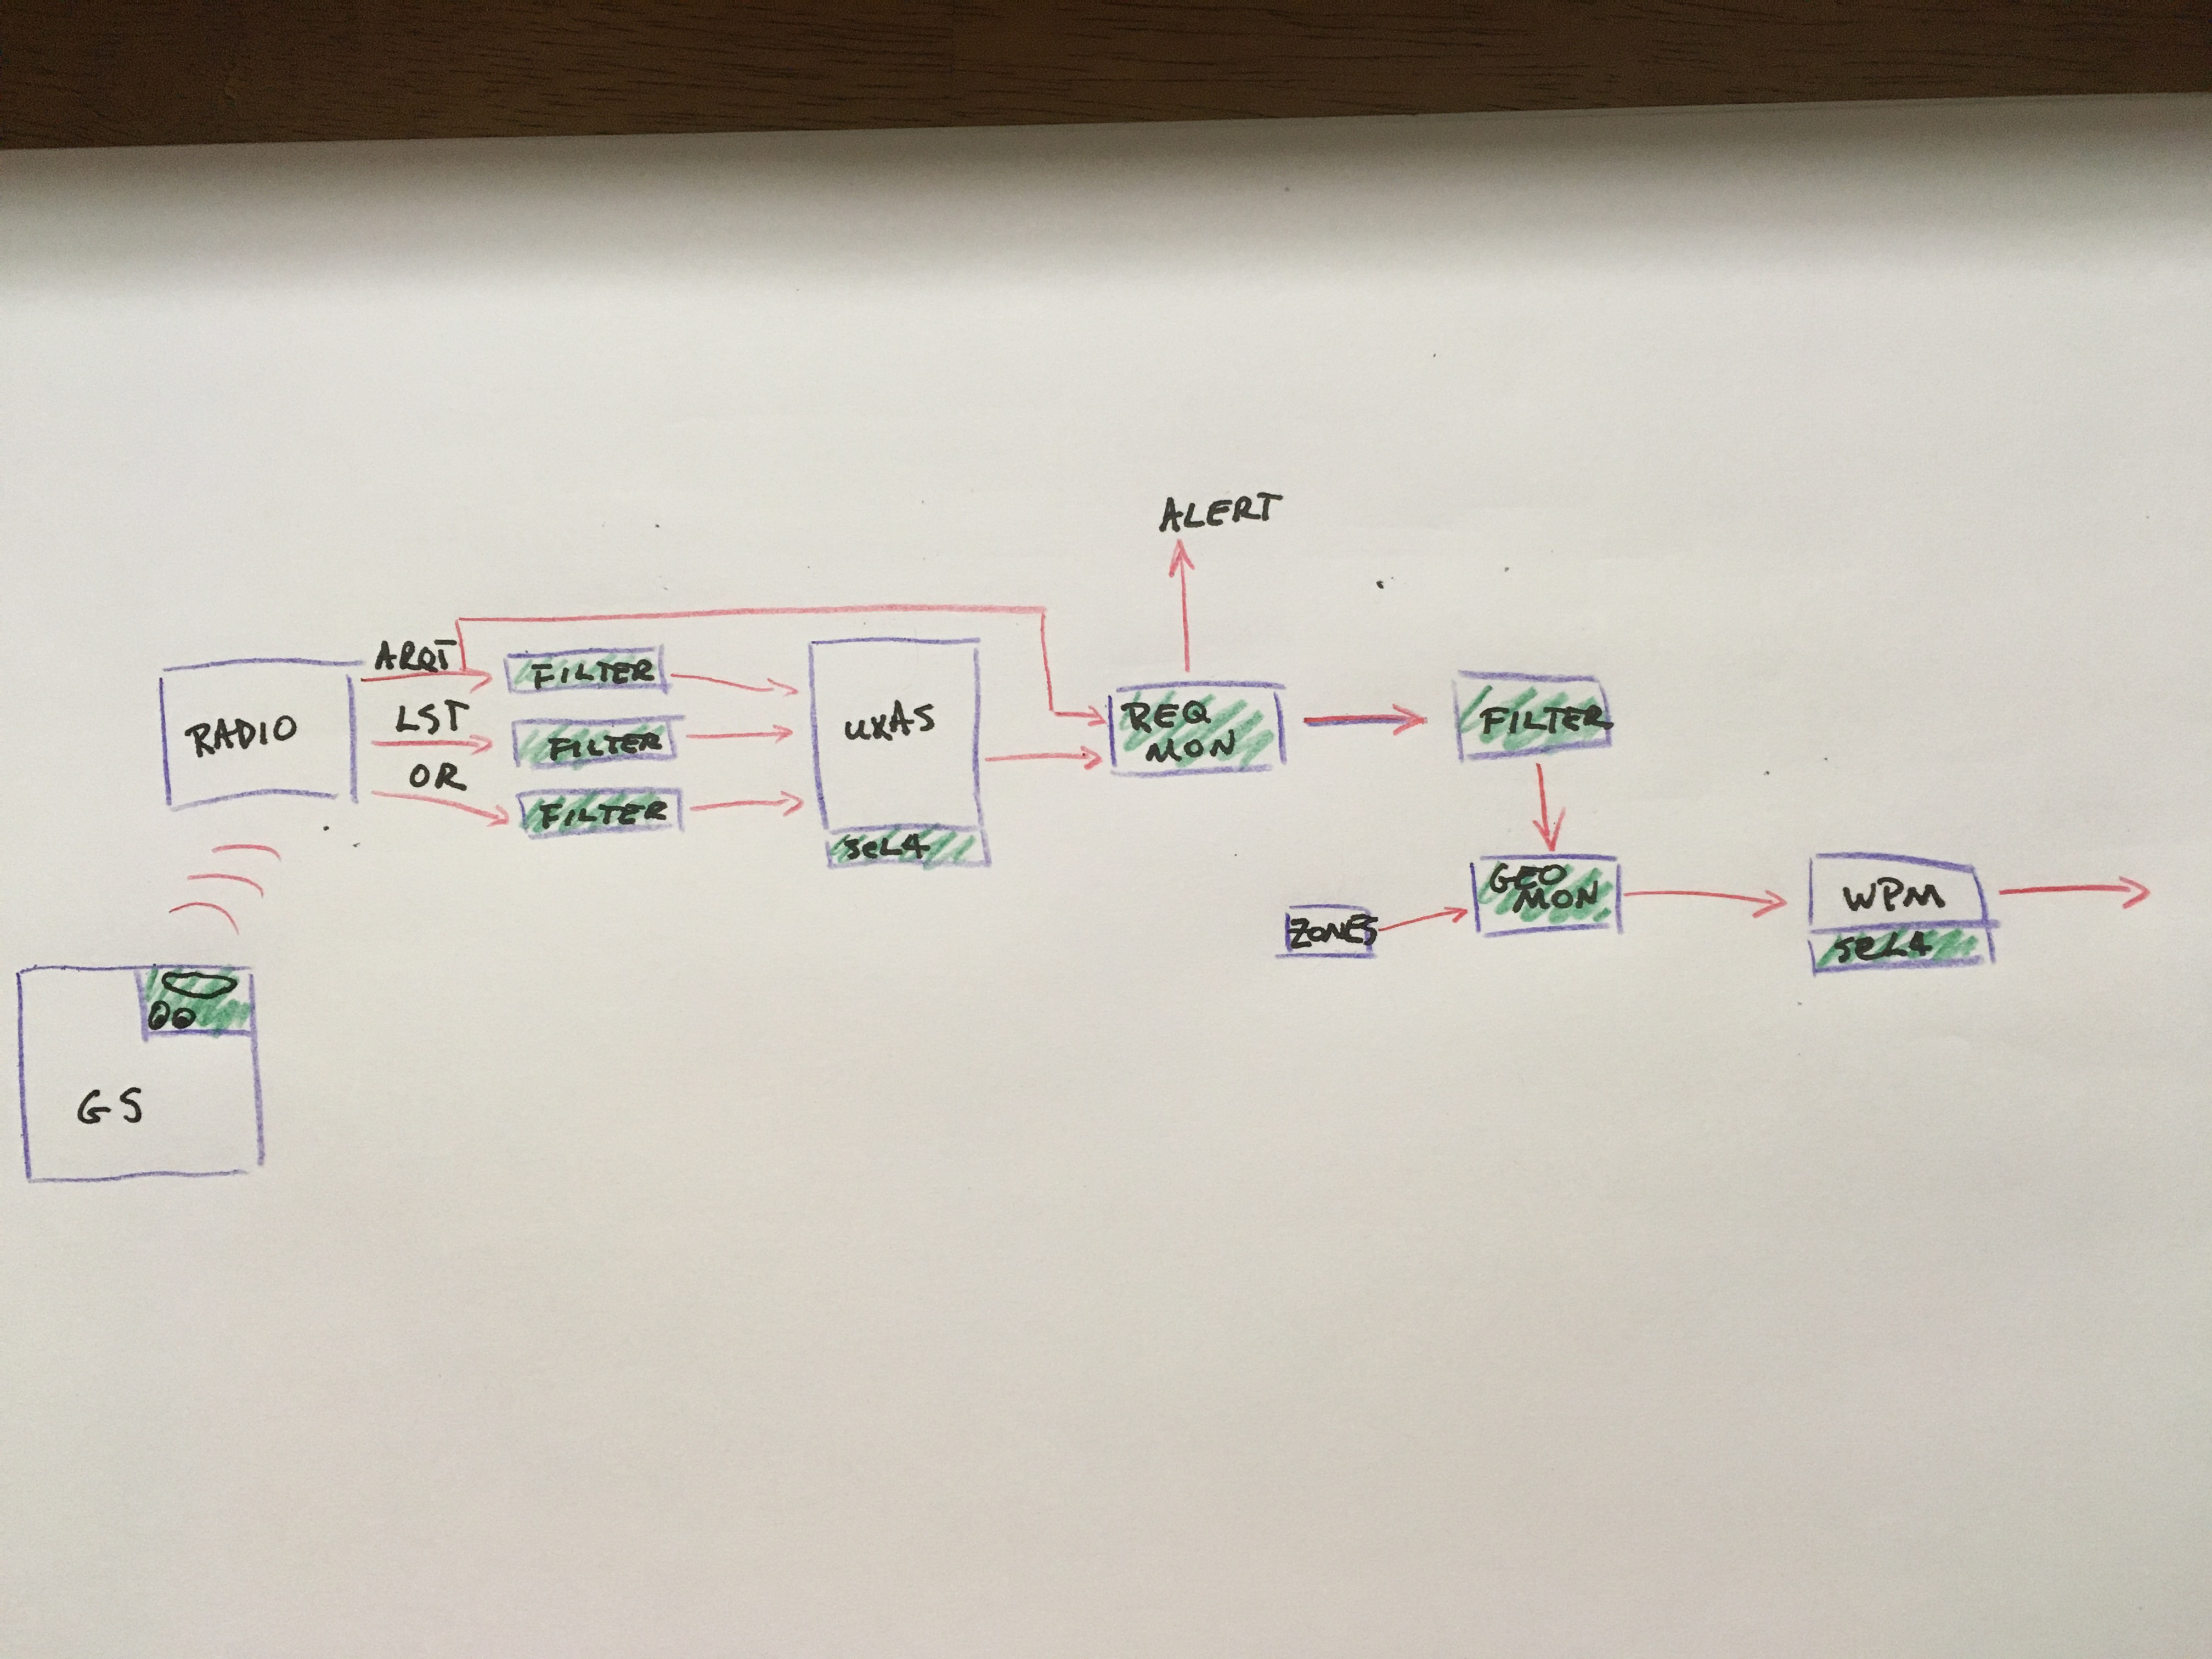
\includegraphics[width=90mm,height=50mm]{final-arch.jpg}


\end{frame}

\begin{frame}\frametitle{Summary}

System designer uses OSATE, using menus to specify and configure transforms.

The interface makes sanity checks and sets up for the eventual system build

Once implementations are created for the new system components, we
have to guard against increasing the attack surface of the system.

Formal specification and proof to the rescue! (Mostly.)

\end{frame}



\section {Deep Dive: Message Filters}

\begin{frame}\frametitle{Ports and Messages}

\begin{itemize}

  \item An AADL component communicates with other components via \emph{connections}

\item  An endpoint (port) on a connection has a \emph{type} (booleans,
  integers, floats, arrays, unions, ...)

\item Properties in AGREE (our specification language) are therefore written over these types.

\item However, in the implementation, messages coming into a port are
  byte arrays (essentially untyped)

\end{itemize}

\end{frame}

\begin{frame}\frametitle{SPLAT}

\begin{itemize}

\item We need to span the gap between high level data and flat strings

\item Our approach : \textbf{SPLAT} (Semantic Properties for Language and Automata Theory)

\item We want to apply ideas from Formal Language Theory to showing
  properties of operations on high-level data.

\end{itemize}

\end{frame}


\begin{frame}[fragile]\frametitle{Example : Wellformed GPS coordinates}

{\small
\begin{verbatim}
 AltitudeType = AGL | MSL

 Location3D = {
  Latitude  : real64,
  Longitude : real64,
  Altitude  : real32),
  AltitudeType : AltitudeType}

 Good_Location (loc) =
    -90.0 <= loc.Altitude <= 90.0 and
   -180.0 <= loc.Altitude <= 180.0 and
      0.0 <= loc.Altitude <= 15000.0
\end{verbatim}
}

\end{frame}

\begin{frame}[fragile]\frametitle{Example : Wellformed GPS message}

{\small
\begin{verbatim}
 Good_Location_String (s) <=>
   exists s1 s2 s3 s4.
      s = concat [s1, s2, s3, s4] and
    -90.0 <= doubleVal(s1) <= 90.0 and
   -180.0 <= doubleVal(s2) <= 180.0 and
      0.0 <= floatVal(s3)  <= 15000.0 and
        0 <= natVal(s4) <= 1
\end{verbatim}
}

where

{\small
\begin{verbatim}
 doubleVal : string -> double
 floatVal  : string -> float
 natVal    : string -> nat
\end{verbatim}
}

\end{frame}

\begin{frame}[fragile]\frametitle{Contiguity Types}

The goal is to automatically generate an implementation of the
well-formedness predicate \verb+Good_Location+ from its specification.

There is a problem : the encoding from datastructures to strings is not specified.

For uxAs, this is a fairly complex encoding.

We specify the message format using \emph{contiguity types}. With this representation we can
\begin{itemize}
\item automatically generate message filters and parsers
\item automatically prove that the filter has the desired property (\verb+Good_Location_String+ in our example)
\end{itemize}

\end{frame}

\begin{frame}\frametitle{uxAS LineSearchTask messages}

 To Be Added

\end{frame}

\begin{frame}[fragile]\frametitle{Contiguity Types: Syntax}

The syntax of contiguity types is very similar to a standard
collection of base types closed under formation of records and arrays.

\[
\begin{array}{rcl}
 \mathit{base} & = & \konst{bool} \mid \konst{char} \mid \konst{u8} \mid
 \konst{u16} \mid \konst{u32} \mid \konst{u64}  \mid \konst{i16} \mid
 \konst{i32} \mid \konst{i64} \mid \konst{f32} \mid \konst{f64} \\
 \tau & = & \mathit{base} \\
      & \mid & \konst{Recd}\; (f_1 : \tau_1) \ldots (f_n : \tau_n) \\
      & \mid & \konst{Array}\; \tau \; \mathit{exp} \\
      & \mid & \konst{Union}\; (\mathit{bexp}_1 : \tau_1) \ldots (\mathit{bexp}_n : \tau_n)
\end{array}
\]
\end{frame}


\begin{frame}[fragile]\frametitle{Contiguity Types: Semantics}

The semantics of contiguity types is in terms of formal languages
(sets of strings):

\[
% \begin{array}{l}
\LangTheta{\tau} =
\mathtt{case}\; \tau\
% \hspace*{3mm}
 \left\{
 \begin{array}{l}
 \mathit{base} \Rightarrow \set{s \mid \konst{len}(s) = \konst{width}(base)} \\
 \konst{Recd}\; (f_1 : \tau_1) \ldots (f_n : \tau_n)
      \Rightarrow \LangTheta{\tau_1} \cdot \ldots \cdot \LangTheta{\tau_n}
\\
 \konst{Array}\; \tau_1 \; \mathit{exp}
      \Rightarrow  \LangTheta{\tau_1}^{\konst{evalExp}\;\theta\;\mathit{exp}}
\\
 \konst{Union}\; (\mathit{bexp}_1 : \tau_1) \ldots (\mathit{bexp}_n : \tau_n) \Rightarrow \\
  \hspace*{5mm}
 \left\{
 \begin{array}{ll}
    \LangTheta{\tau_i} &  \mathrm{if}\ \konst{evalBexp}\;\theta\;\mathit{bexp}_i = \konst{true} \\
                  & \mathrm{and\ no\ other}\ \mathit{bexp}_j\ \mathrm{is}\ \konst{true}  \\
    \emptyset & \mathrm{otherwise}
 \end{array}
 \right.
 \\
\end{array}
 \right.
%\end{array}
\]
\end{frame}

\begin{frame}[fragile]\frametitle{Correctness of parameterized matcher}

We can define a function \textbf{match} which takes a contig type and
a string and returns an assignment of slices of the string to elements of the type.

\begin{theorem}[Correctness]
  \[
  \konst{match}\; \mathit{contig}\; \mathit{string} = \konst{Some}(\theta) \imp
   \mathit{string} \in \LangTheta{\mathit{contig}}
\]
\end{theorem}

\textbf{match} has the flavor of a \emph{parser generator}: it takes a
specification of the language to be parsed and returns an implementation

We use \textbf{match} to implement all filters in the transformed uxAS
and parsers for the monitors.

\end{frame}

\section {Security Case}

\begin{frame}\frametitle{Joining theorems together}

  We can join the correctness of the message matcher with the
  correctness of the CakeML toolchain to obtain a \emph{single-shot} correctness theorem in HOL4:

  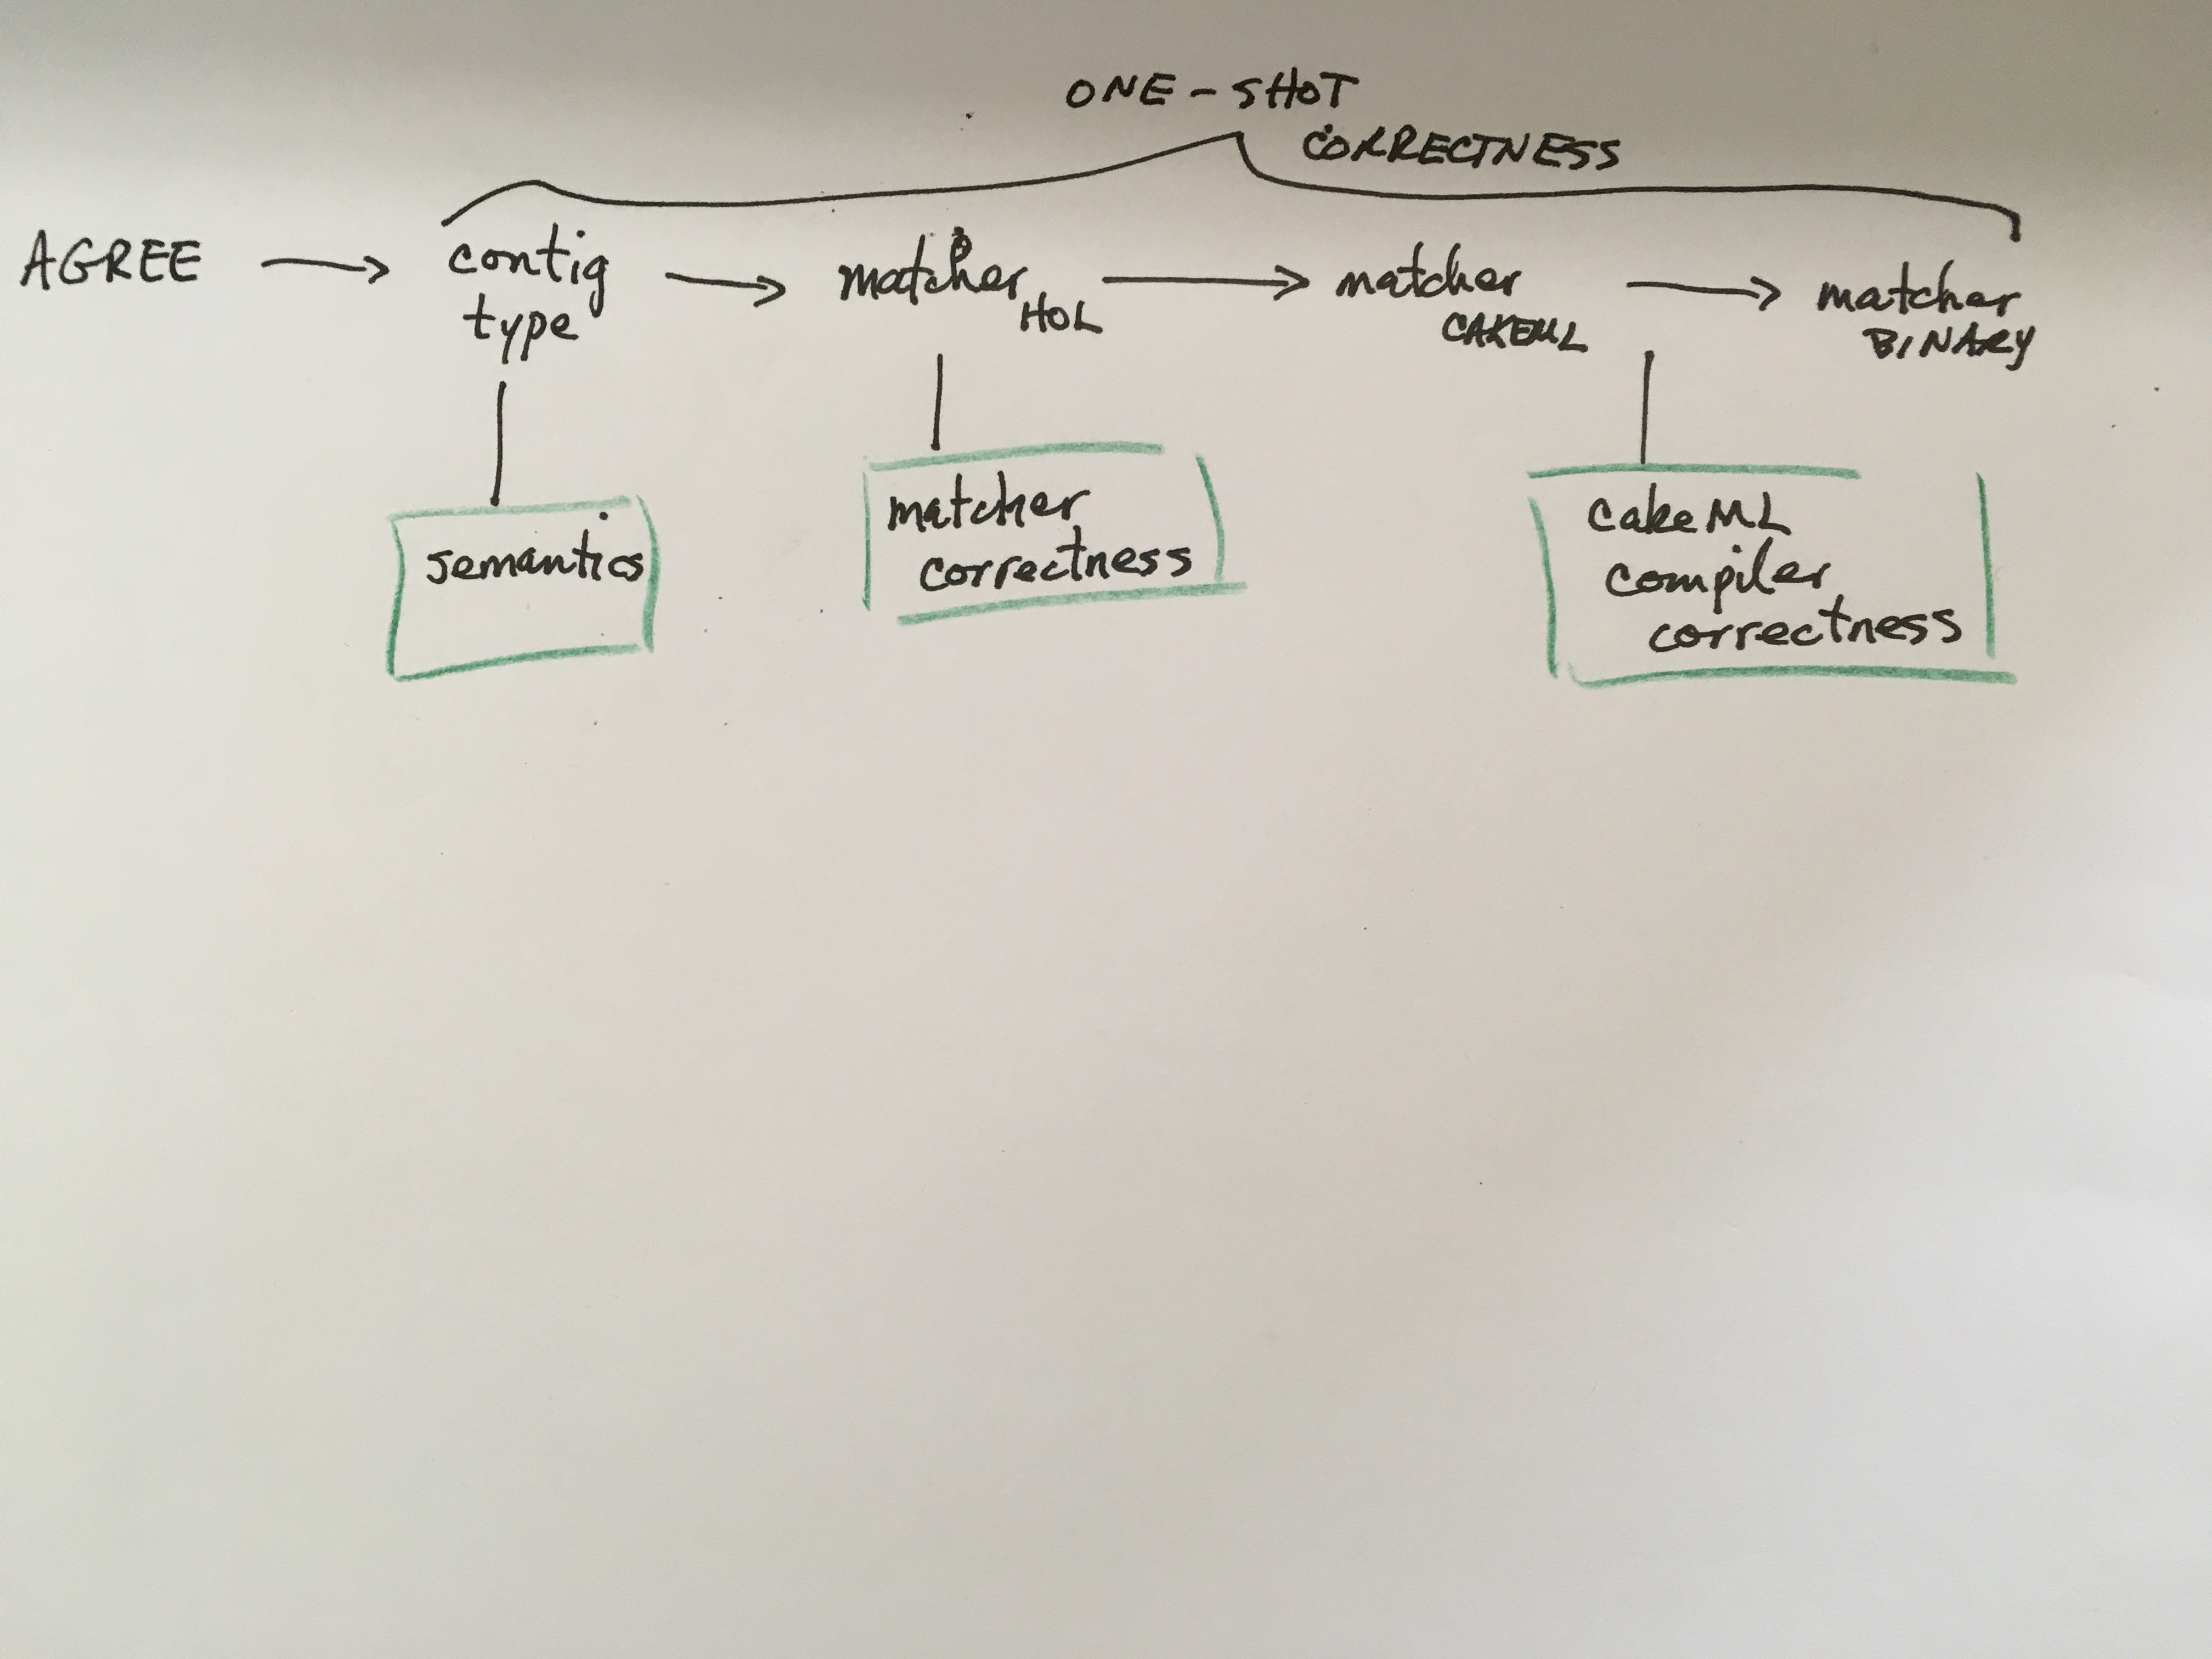
\includegraphics[width=90mm,height=50mm]{one-shot.jpg}

\end{frame}


\begin{frame}\frametitle{Thread level correctness}

  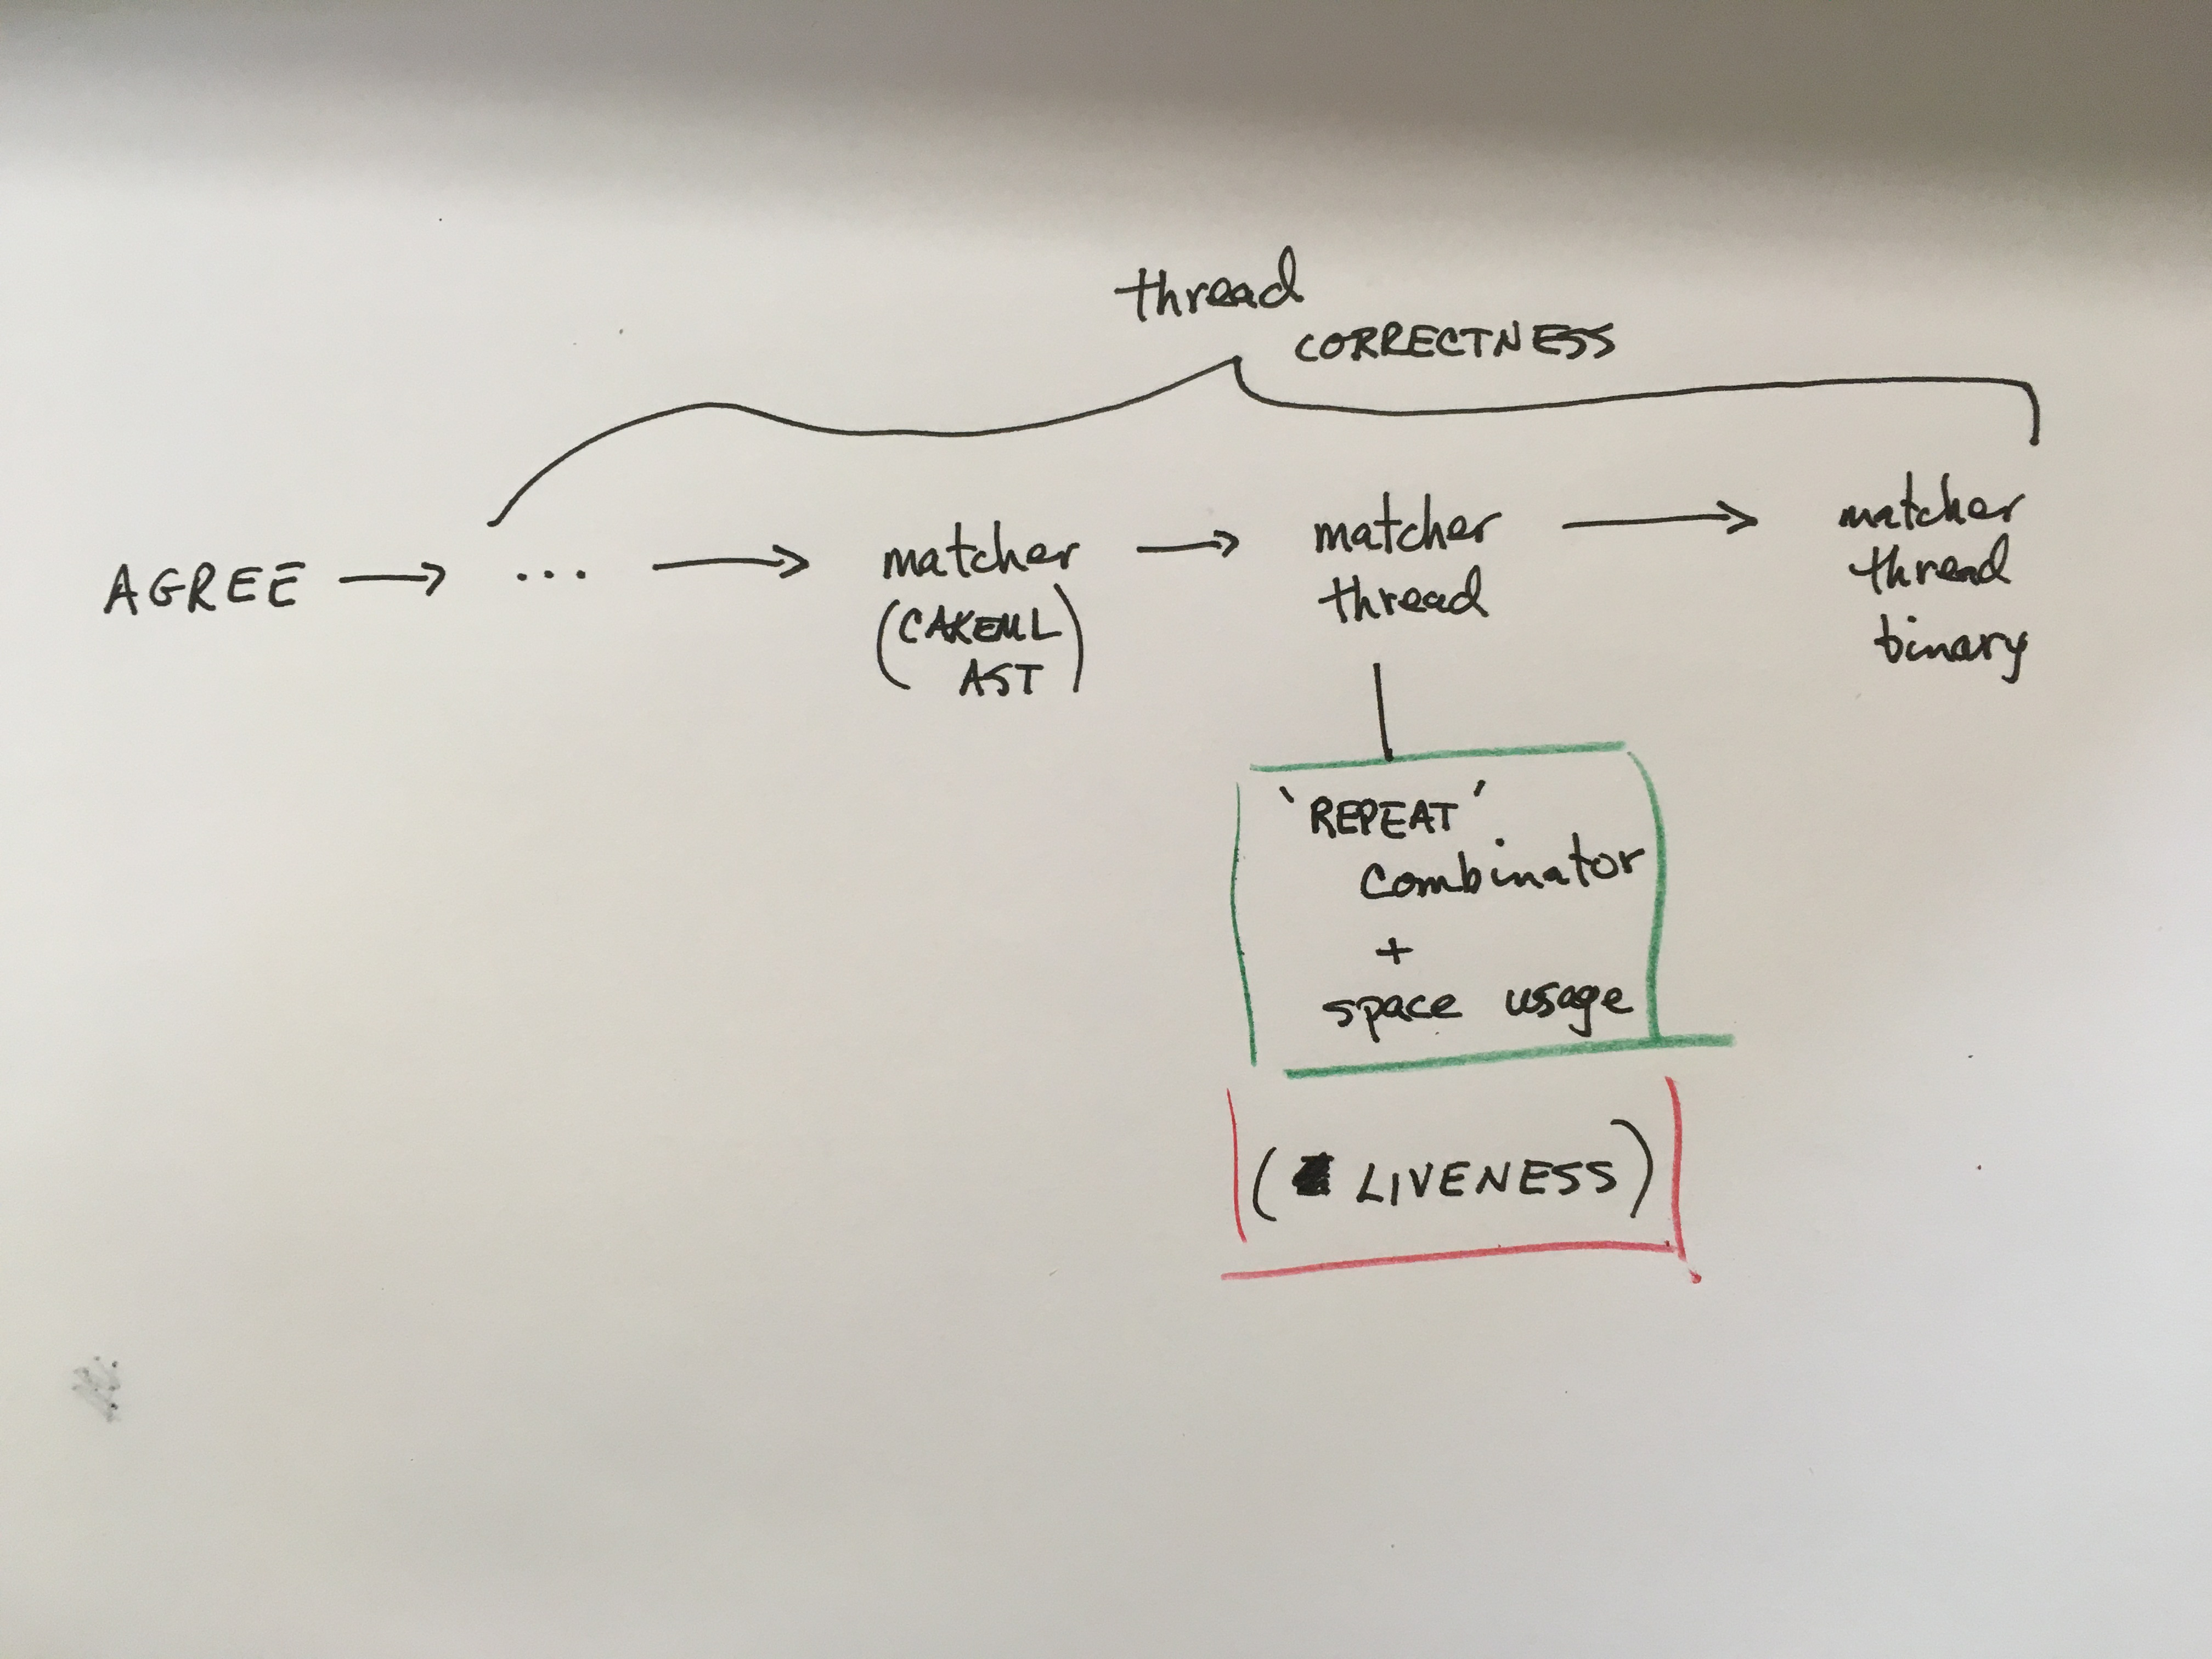
\includegraphics[width=90mm,height=50mm]{thread.jpg}

\end{frame}

\begin{frame}\frametitle{System-level correctness}

Recall \textbf{NEAT}:
  \begin{itemize}
   \item Non-bypassable
   \item Evaluable
   \item Always invoked
   \item Tamper proof
 \end{itemize}

  Desirable properties for our implementation!

We already `have' some of these :

  \begin{itemize}
   \item Non-bypassable
   \item Evaluable (Proofs)
   \item Always invoked (Liveness)
   \item Tamper proof (seL4)
 \end{itemize}

\end{frame}

\begin{frame}\frametitle{System-level correctness}

Note: Non-Bypassability is a system-wide property which depends on the
implementation rigorously obeying the boundaries in the model

Also the vast iceberg of the security properties that seL4 implements
need to be brought into the picture.

Problem: Disparate evidence supporting our security claim.

Solution: Represent the security argument in Resolute

\end{frame}


\begin{frame}\frametitle{Comments and TODO}

\begin{itemize}
\item Start off by giving thanks to the organizers
\item Goes too fast into details; give a more gradual approach to SysArch concept
\item Slide 12 (too many acronyms)
\item Too much text (needs more pictures)
\item Use material from earlier presentations from Isaac and Darren
\item ``Now we implement'' Mark a definite shift from transformations to implementations.
\item Define Tamper-proof
\item Explain ``What is the significance of end-to-end correctness proofs?''
\item Role of HAMR + Adventium stuff
\item Shout-outs to both Kansas places.

\item Be crisper on Non-Bypass vs Always invoked (AInv is not
  liveness; it's liveness plus the fact that it obeys its spec (by
  output being equal to filter function applied to its input)). In
  other words, the filter function can't just output well-formed data:
  the output stream has to be the filtered input stream.

\item Try to express the entire assurance case in a picture: ``it's
  the original system, except safer in the following ways''

\item Map from AADL-->Camkes-->seL4
\item Where we are; what's next

\end{itemize}
\end{frame}

\end{document}
